%*******************************************************************
%   Project Name: BracU Thesis Template
%   Prepared by: Ayesha Abed Library, Brac University
%   
%   "Predicting a T20 Cricket Match Result While The Match is in Progress", this thesis was 
%   submitted to BracU on 23 August, 2015 by Fahad Munir, Md. Kamrul Hasan, Sakib Ahmed, Sultan Md. Quraish
%   Authors have given full consent to use their thesis as a sample to develop a Thesis Template using LaTex 
%   PLEASE KEEP ALL FILES IN THEIR DESIGNATED FOLDERS
%*******************************************************************
% Project Structure:
% appendix: Contains “appendix.txt” files.
% bibliography: Contains “references.bib” file.
% chapters: Contains “chapter.txt” files. For every chapter, create separate “chapter_[1,2,3..].txt” files.
% core: This folder will contain following files:
%     declaration.txt
%     approval.txt
%     ethics_statement.txt
%     abstract.txt
%     dedication.txt
%     acknowledgement.txt
%     titlepage.txt
% images:Contains all images files. 
% main.txt
%     This is the main.txt file. All the packages and environment variable are declared in main.txt. All others .txt files are referred from this file.
%
% If you have any questions or concerns about the latex template, please feel free to visit Ayesha Abed Library.
%*******************************************************************

\documentclass[Times,12pt,oneside,openany,print,index]{report}
\usepackage[a4paper,width=150mm,top=25mm,bottom=25mm]{geometry}
\usepackage[english]{babel}
\usepackage[utf8]{inputenc}
\usepackage{csquotes} % Provides advanced facilities for in-line and display quotations
\usepackage{amsmath} % TO use mathematical equations 
\pagestyle{plain} % Just a plain page number. For more http://www.emerson.emory.edu/services/latex/latex_129.html

\usepackage{graphicx} % to use the graphicx package
\graphicspath{/images} % Path to Image files 
\usepackage{caption} % To use caption with figure and images
\usepackage{array} % The array environment is used to make a table of information, with column alignment (left, center, or right) and optional vertical lines separating the columns

\usepackage[nottoc]{tocbibind} % The tocbibind package can be used to add the ToC and/or bibliography and/or the index etc., to the Table of Contents listing

\usepackage[normalem]{ulem} % The ulem package provides various types of underlining that can stretch between words and be broken across lines.

\usepackage[backend=biber,style=ieee,sorting=ynt]{biblatex} % for more plz click https://www.overleaf.com/learn/latex/Biblatex_citation_styles
\addbibresource{bibliography/references.bib} % Imports bibliography file

\usepackage{hyperref} % Provides LaTeX the ability to create hyperlinks within the document.
\hypersetup{
    colorlinks=true,
    linkcolor=black,
    filecolor=magenta,      
    urlcolor=black,
    citecolor=black,
}
\urlstyle{same}

\setlength{\parindent}{0em} % To control Indentation of paragraphs 
\setlength{\parskip}{5pt} % adds 5pt after every paragraph

\usepackage{nomencl} % The nomenclature package can be used to generate and format a nomenclature using MakeIndex.
\renewcommand{\nompreamble}{The next list describes several symbols \& abbreviation that will be later used within the body of the document}
\makenomenclature

\let\cleardoublepage=\clearpage % removes unwanted doublepages

\usepackage{graphicx} % to use the graphicx package
\graphicspath{/images} % Path to Image files 
\usepackage{caption} % To use caption with figure and images
% correct bad hyphenation here
\hyphenation{op-tical net-works semi-conduc-tor}

\usepackage[dvipsnames]{xcolor}
\definecolor{astral}{RGB}{46,116,181}
%
\usepackage{caption}
\usepackage{comment}
\usepackage{hyperref}
\usepackage{amsmath} % For better mathematical typesetting
\usepackage{textalpha}
\usepackage{tabularx} % Add this to your preamble
\usepackage{multirow}
\usepackage{graphicx}
\usepackage{array}
\usepackage{tabularx}
\usepackage{calc} % For width calculations
\usepackage{amssymb}  % For \mathbb
\usepackage{booktabs}
\usepackage[style=ieee]{biblatex}
\usepackage{tikz}
\usetikzlibrary{positioning, arrows.meta, shapes.geometric, calc, fit, backgrounds}

% --- Algorithms (correct combo) ---
\usepackage{algorithm}
\usepackage[noend]{algpseudocode} % noend optional

% --- Make sure enumitem doesn't hijack labels inside algorithms ---
\usepackage{enumitem}
\SetEnumitemKey{algfix}{label=\arabic*.,leftmargin=*,align=left}
% algpseudocode doesn't use enumerate, but if something else does, this prevents a,b,c labels.

% --- Nicer line numbers & keyword casing ---
\algrenewcommand\alglinenumber[1]{\footnotesize #1}
\algrenewcommand\algorithmiccomment[1]{\hfill\(\triangleright\)~#1}
\algrenewcommand\textproc{\textsc} % \textproc{Foo} -> small caps

% Title-case some printed keywords (optional):
\makeatletter
\renewcommand{\ALG@name}{Algorithm} % caption name
\makeatother

\begin{document}

\thispagestyle{empty} % removes page number from title page

\begin{titlepage}
\renewcommand*{\thepage}{Title} % Change page number in PDF

    \begin{center} 
        \vspace*{3cm} % For creating Vertical Blank Space
        
        {\fontsize{16pt}{22pt}\selectfont{Combining Reconstruction and Non-Heuristic Joint-Embedding Learning for Bengali Speech}
        } % "fontsize{font size}{line space}\selectfont{}" command to override font size and line space for the Title
        
        \vspace{1.5cm}
        
        \text{by}
        
        \vspace{0.5cm}
        
        	Tamanna Afroz\\
	        23366033\\

        \vspace{1.5cm}
        
        	A thesis submitted to the Department of Computer Science and Engineering\\
            in partial fulfillment of the requirements for the degree of\\
            M.Sc. in Computer Science \& Engineering

        
        \vspace{2.5cm}
        
    		Department of Computer Science and Engineering\\
            BRAC University\\
            September 2026
        
        \vspace{3cm}
        
    		\copyright\ 2026. BRAC University\\
            All rights reserved.
    
    \end{center}

\end{titlepage} % Add title page
\cleardoublepage

\pagenumbering{roman} % Roman numbers to be use all pages before Chapter 1

%*******************************************************************
% TOC = Table of Contents
% The hyperref makes Title page No. 1 entry in the TOC
% In order to properly link  all section in TOC "phantomsection" command used
%  see below link for details on "addcontentsline"
% http://www.emerson.emory.edu/services/latex/latex_162.html
% "input" command to add files
% "Ethics Statement" & "Dedication" page are Optional; you may omit this two page if you want
% Please do not change the order of listings in TOC
%*******************************************************************
\phantomsection
\addcontentsline{toc}{chapter}{Declaration}
% Following command is used to created grouped signature line for Four Authors
\newcommand*\wildcard[2][6cm]{\vspace{2cm}\parbox{#1}{\hrulefill\par#2}} 

% A "parbox{}{}" is a box whose contents are created in paragraph mode. 
% "hrulefill{} to chance thickness of underline"

\section*{Declaration}

It is hereby declared that

\begin{enumerate} % begin{enumerate} function to create numbered list
  \item The thesis submitted is my/our own original work while completing degree at BRAC University.
  \item The thesis does not contain material previously published or written by a third party, except where this is appropriately cited through full and accurate referencing.
  \item The thesis does not contain material which has been accepted, or submitted, for any other degree or diploma at a university or other institution.
  \item We have acknowledged all main sources of help.
\end{enumerate}

\vspace{1cm}
\textbf{Student’s Full Name \& Signature:} % Testbf{} for Bold

\begingroup

    \begin{center}
        \wildcard{\centering Tamanna Afroz \\ 23366033}
    \end{center}

\endgroup


\pagebreak







\phantomsection
\addcontentsline{toc}{chapter}{Approval}
\section*{Approval}

The thesis/project titled “BanglaSpeechFM: Towards a Foundation Model for Bangla Speech” submitted by 
\begin{enumerate}
  \item Tamanna Afroz (23366033)
\end{enumerate}

Of Fall, 2025 has been accepted as satisfactory in partial fulfillment of the requirement for the degree of M.Sc. in Computer Science on November 9th, 2025.

\vspace{0.5cm}
\textbf{Examining Committee:}

\vspace{1cm}

Examiner:\\
(External)
\begin{center}
    \hspace{7cm} \wildcard{\centering Name \\ Professor\\ Department of Computer Science and Engineering\\ BRAC University } \hspace{1cm} 
\end{center}

Examiner:\\
(Internal)
\begin{center}
    \hspace{7cm} \wildcard{\centering Name \\ Professor\\ Department of Computer Science and Engineering\\ BRAC University } \hspace{1cm} 
\end{center}

Supervisor:\\
(Member)
\begin{center}
    \hspace{7cm} \wildcard{\centering Md. Golam Rabiul Alam, PhD \\ Professor\\ Department of Computer Science and Engineering\\ BRAC University } \hspace{1cm} 
\end{center}

Program Coordinator:\\
(Member)
\begin{center}
    \hspace{7cm} \wildcard{\centering Md Sadek Ferdous, PhD \\ Professor\\ Department of Computer Science and Engineering\\ BRAC University } \hspace{1cm}
\end{center}

Head of Department:\\
(Chair)
\begin{center}
    \hspace{7cm} \wildcard{\centering Sadia Hamid Kazi, PhD \\ Chairperson and Associate Professor\\ Department of Computer Science and Engineering\\ BRAC University } \hspace{1cm}
\end{center}

\pagebreak

% \phantomsection
% \addcontentsline{toc}{chapter}{Ethics Statement}
% \input{core/ethics_statement}

\phantomsection
\addcontentsline{toc}{chapter}{Abstract}
\section*{Abstract}
Botnets pose a significant cybersecurity threat, enabling attacks such as DDoS, data theft, and service disruptions on IoT devices. These devices often lack built-in botnet traffic filtering, leaving them highly exposed. Existing AI-based solutions improve detection capabilities but have limitations: (i) they are too heavy for IoT deployment, and (ii) they lack unlearning capabilities to forget sensitive or outdated features without retraining. To address these challenges, we propose DiRLU, a lightweight, reinforcement learning driven framework, while ensuring privacy by selectively unlearning sensitive or outdated features without requiring retraining. The framework leverages knowledge distillation to transfer knowledge from a teacher model into a lightweight student model, with both models trained using A2C. A post-hoc unlearning mechanism modifies weights to remove targeted features, while restored features show negligible performance loss, confirming reversibility. Unlike many benchmark models that used only 5\% of the BoT-IoT dataset, this research leverages 25\%, allowing us to develop a strong teacher model. Both the teacher and student models were trained using the A2C reinforcement learning algorithm, achieving impressive results, with the student model achieving 99.60\% accuracy and a 99.80\% F1 score. To enhance transparency, we integrated Explainable AI (XAI), particularly LIME, which helps interpret the model’s decisions and identify the key features influencing its predictions. DiRLU combines efficiency with privacy, aligning with GDPR standards (right to be forgotten) to provide practical IoT security. By combining knowledge distillation, feature unlearning and XAI, this research not only strengthens botnet detection but also sets new standards for security, interpretability, and data privacy in cybersecurity.

\vspace{1cm}
\textbf{Keywords:} Botnet, Reinforcement Learning, Feature Unlearning, Knowledge Distillation, Explainable AI, A2C, Security \& Privacy
\pagebreak


% \phantomsection
% \addcontentsline{toc}{chapter}{Dedication}
% \input{core/dedication}

\phantomsection
\addcontentsline{toc}{chapter}{Acknowledgment}
\section*{Acknowledgement}
Firstly, all praise to the Great Allah, by whose grace our thesis has been completed. We express our heartfelt gratitude to our supervisor Professor Golam Robiul Alam Sir for his kind support, valuable guidance, feedback and constant encouragement throughout this work. Our appreciation goes to the Department of Computer Science and Engineering of BRAC University for providing the necessary facilities and support.

\renewcommand{\contentsname}{Table of Contents} % Rename TOC name from Contents to Table of Contents
\cleardoublepage
\phantomsection
\addcontentsline{toc}{chapter}{Table of Contents} % Add Table of Contents in TOC
\tableofcontents % To  generation of the Table of Contents

\listoffigures % To  generation of the List of Figure
\listoftables % To  generation of the Tables of Figure

\printnomenclature % TO  generation of the Nomenclature file
\addcontentsline{toc}{chapter}{Nomenclature}
\cleardoublepage

\pagenumbering{arabic} % To use page number 1,2,3 ..

\chapter{Introduction}
%\section{Introduction}
Speech representation learning has seen remarkable progress with the advent of self-supervised learning (SSL) techniques, enabling the development of foundation models capable of understanding and processing human speech. While state-of-the-art (SOTA) speech models have achieved unprecedented success in high-resource languages, low-resource languages like Bengali often suffer from a lack of dedicated, efficient models built from scratch. Most existing works in Bengali speech AI rely on fine-tuning massive, pre-trained multilingual models, which are computationally expensive and not optimized specifically for the linguistic nuances of Bengali. Furthermore, the immense size of these SOTA models limits their deployability in resource-constrained environments. This research addresses this gap by developing an AI/ML speech foundation model specifically for Bengali, trained entirely from scratch using self-supervised learning on publicly available datasets. By doing so, we demonstrate that training a compact, dedicated model from scratch is not only viable but can also yield highly effective representations for Bengali speech.

\section{Problem Statement}
Despite the growing interest in speech technologies, there is a significant scarcity of foundational speech models built from scratch for the Bengali language. Current approaches predominantly involve fine-tuning extremely large SOTA models trained on other languages or multilingual corpora. This reliance on massive pre-trained models presents two major challenges: first, the computational cost and memory footprint of these models make them impractical for widespread deployment or research with limited resources; second, they often lack specialized adaptation to the unique phonetic and phonological characteristics of Bengali. There are currently no researchers who have successfully developed a small-scale, highly efficient speech foundation model for Bengali from scratch using self-supervised learning on public datasets. Therefore, there is a critical need to investigate whether a significantly smaller, dedicated model can be trained from scratch to achieve competitive or superior performance in specific metrics compared to existing heavy-weight SOTA models.

\section{Thesis Objective}
The primary objective of this thesis is to design, train, and evaluate a Continuous Latent Encoder (CLE) for Bengali speech representation learning. By developing a compact speech foundation model from scratch using self-supervised learning techniques, we aim to provide a highly efficient alternative to fine-tuning large SOTA models. The specific objectives of this research are summarized as follows:

\begin{itemize}
    \item To develop a lightweight speech foundation model (a 23.8M-parameter continuous-latent autoencoder) specifically tailored for 16 kHz Bengali speech using publicly available datasets.
    \item To demonstrate that training a model from scratch using self-supervised learning is a viable and highly effective pathway for Bengali speech research, eliminating the strict dependency on fine-tuning massive multilingual models.
    \item To evaluate the performance of the proposed compact model and show that despite its significantly small size compared to SOTA speech models, it achieves superior results in specific evaluation metrics.
    \item To provide a robust, frame-level speech representation that can be utilized for various downstream Bengali speech analysis tasks, establishing a foundation for future research in low-resource language speech AI.
\end{itemize}

\section{Thesis Outline}
The rest of the paper has been organized as follows: Chapter-\hyperref[related_work]{2} explains some relevant research in speech foundation models and self-supervised learning, along with their contributions and limitations. Chapter-\hyperref[methodology]{3} describes the methodology, dataset, and the continuous-latent autoencoder architecture used in this research in detail. Chapter-\hyperref[result_and_analysis]{4} presents the results we obtained from this study, including comparative analyses with SOTA models to evaluate the effectiveness of our approach. We also describe some limitations and future goals of this paper. Finally, in Chapter-\hyperref[conclusion]{5}, we conclude the thesis, providing the study's findings and potential areas for further exploration.

% \nomenclature{$ODI$}{One day International}
% \nomenclature{$T20$}{Twenty Twenty}
% \nomenclature{$ODI$}{One day International}
% \nomenclature{$IPL$}{Indian Premier League}
% \nomenclature{$ODI$}{One day International}
% \nomenclature{$MR$}{Runs scored by Home team}
% \nomenclature{$OR$}{Runs scored by the opponent team}
% \nomenclature{$MRN$}{Home Team Run Rate}
% \nomenclature{$ORN$}{Opponent Team Run Rate}
% \nomenclature{$LBW$}{Leg before Wicket}

\chapter{Related Work}\label{related_work} 
Several related studies have already been conducted to detect Botnet network traffic. This section briefly summarizes some studies and their approaches to detecting Botnet network traffic.

%Detecting Information Theft Attacks in the Bot-IoT Dataset [1]
Leevy et al. \cite{n3} build a successful predictive machine learning model for detecting information theft attacks. This study used eight ML classifiers (four ensembles and four non-ensembles) and two evaluation metrics (AUC and AUPRC). The authors used only six features of the Bot-IoT dataset to get only specific insights about information theft attacks. The authors used 556 instances and other cutting-edge technologies, such as k-fold cross-validation, for training the model. Based on AUC and AUPRC results, the ensemble classifiers performed better than the non-ensemble classifiers. However, the LightGBM ensemble classifier performed top among all; it exhibited AUC results of 98\% and AUPRC of 99\%.

%Towards the Development of Realistic Botnet Dataset in the Internet of Things for Network Forensic Analytics: Bot-IoT Dataset [2]
Koroniotis et al. \cite{n4} proposed a dataset, Bot-IOT, to simulate different types of network attacks, such as probing attacks, DDoS, DoS, and Information theft. Authors build the dataset to address other datasets' drawbacks with accurate labeling and incorporate recent attacks. They captured one GByte raw packet to extract complete information on network features. They introduced 32 features and created ten other hybrid features for simulation and testing the dataset's accuracy. They also evaluated the reliability of the dataset using ML (SVM) and deep learning algorithms (RNN and LSTM). SVM performed best with a full-featured dataset and scored 99\% accurately, whereas RNN and LSTM performed 99\% accurately with the ten best features only.

%An Intrusion Detection System Using BoT-IoT
Alosaimi et al. \cite{n5} developed a machine learning-based intrusion detection system to secure IOT applications. The authors used the BOT-IoT dataset and a combination of deep learning and machine learning algorithms to train and test the model. The authors only used four files of the dataset, containing only 5-6\% of the dataset. The first file contains only a DoS attack, the second one includes a DoS and DDoS attack, The third one contains two DDoS attacks, and The fourth one contains many attacks. They evaluated the results using accuracy, error rate, recall, and specificity. However, in the second database, the ensemble bag algorithm acquired an accuracy of 100\% at all levels of the database, while the decision tree obtained an accuracy of 100\% at all levels of the database in the third database. This study demonstrates remarkable improvements in intrusion detection, especially DoS attacks, compared to existing models.

%A Novel Method for Malware Detection Using Audio Signal Processing Techniques
Farrokhmanesh et al. \cite{n6} designed a new machine learning-based model for detecting malicious activity in computers and networks. The authors proposed their model, which is based on audio signal processing techniques. They represented binary bytes as audio signals and applied MIR techniques for detecting malware. The authors used 3400 samples containing both malware and benign, however, they used the VX Heavens dataset for malware and Windows XP files for benign. They used KNN, AdaBoost, and Random Forest classifiers, among them AdaBoost performed best in terms of accuracy (92.2\%). The authors demonstrated a lightweight novel model with good accuracy and is computationally efficient.

%A survey of malware detection using deep learning
Bensaoud et al. \cite{n7} arranged a survey to examine how deep learning (DL) detects malware across multiple operating systems, including MacOS, Windows, iOS, Android, and Linux. They investigate different Deep Learning techniques, including text and image classification, pre-trained models, and multi-task learning, to determine how well they detect malware software. The paper also highlights significant problems, such as defined benchmark datasets, the complexity of deep learning models, and their sensitivity to adversarial attacks. It also emphasizes the value of Explainable AI (XAI) in making these models more transparent and intelligible. This study provides valuable insights into malware detection techniques by testing eight deep-learning approaches on various datasets.

%Machine Unlearning: A Comprehensive Survey
Wang et al. \cite{n8} discuss the concept of machine unlearning, which focuses on enabling a trained model to remove or “forget” certain data. Their survey reviews different approaches, ranging from straightforward methods like deleting data and retraining, to more sophisticated gradient-based techniques that adjust the model without full retraining. They compare these strategies in terms of efficiency, computational cost, and impact on model accuracy. The study also highlights the challenges of ensuring that unlearning is applied reliably while still maintaining overall model performance. It identifies gaps in existing research, such as the need for consistent benchmarks. This paper proposes future ideas for increasing the scalability and usability of unlearning in large-scale machine-learning applications.

%A Lightweight Malware Detection Model Based on Knowledge Distillation
Miao et al. \cite{n9} propose DistillMal, a novel strategy for improving malware detection efficiency via a knowledge distillation architecture. The basic concept is to train a compact student network to replicate the performance of a more extensive, complex teacher network, resulting in a lightweight model suitable for deploying devices with limited resources. Extensive testing on two new datasets demonstrated that the student network performs similarly to the teacher model. The student model obtained 94.5\% detection accuracy, compared to 95\% for the teacher model, while lowering the number of parameters by 60\% and the inference time by 50\%. This demonstrates that DistillMal efficiently balances model size and detection accuracy. By leveraging knowledge distillation, the proposed method addresses the challenges of deploying large-scale deep learning models in environments with limited computational resources, such as mobile devices or IoT systems.

%Explainability in AI-based behavioral malware detection systems
Galli et al. \cite{n10}, in their work "Explainability in AI-based behavioral malware detection systems," highlight the growing need for transparency in machine learning models that track behavior patterns to detect malicious software. To address this, they designed a detection model that incorporates interpretability tools such as SHapley Additive exPlanations (SHAP), which help show how individual features influence the model’s decisions. This allows cybersecurity professionals to see which behavioral indicators play the most important role in classifying software as malicious or benign. Their approach achieved high accuracy, demonstrating strong malware detection performance. By combining explainability with detection, the system not only improves threat response but also builds trust and supports regulatory requirements. The study underscores the importance of striking a balance between powerful detection capabilities and clear, understandable AI-driven insights.

%Machine Learning-Based Early Detection of IoT Botnets Using Network-Edge Traffic
Kumar et al. \cite{n11} introduced EDIMA, a lightweight approach designed for early detection of IoT botnets at home network edge gateways. The framework combines traffic classification with Autocorrelation Function (ACF)-based testing to spot signs of bot activity. Their results show that EDIMA can accurately identify bot scanning and command-and-control (CnC) traffic, achieving a detection rate of 98\% while maintaining a low rate of false positives. As the number of IoT devices rises, their performance stays strong. When authors use a Raspberry Pi, EDIMA exhibits short detection delays and low resource usage. The technology works better than current botnet-related traffic detection techniques. Furthermore, there is no appreciable processing penalty when EDIMA is implemented in real-time on edge devices. The technique provides scalable and efficient security against botnet threats in IoT environments.

%PAIRED: An Explainable Lightweight Android Malware Detection System
To effectively identify Android malware and provide results that can be explained, the paper "PAIRED: An Explainable Lightweight Android Malware Detection System" introduces PAIRED \cite{n12}. To find malicious programs, PAIRED combines machine learning and static analysis methods. The system's ability to differentiate between dangerous and benign programs is demonstrated by its 94\% detection accuracy. Furthermore, PAIRED is appropriate for deployment on devices with constrained computing capabilities due to its lightweight architecture, which guarantees that it uses few resources. By using explainable AI algorithms, consumers may comprehend the characteristics that go into a detection judgment. The increasing security threats brought on by the extensive use of Android smartphones are addressed by PAIRED, which provides both explainability and excellent detection rates.

%Assessing LLMs in malicious code deobfuscation of real-world malware campaigns
Patsakis et al. \cite{n13} investigated the use of Large Language Models (LLMs) for deobfuscating malicious code, focusing on the Emotet malware campaign. Their study tested four different LLMs to see how well they could interpret and simplify obfuscated code. The results showed that, although the models struggled with more advanced obfuscation techniques, they were able to successfully recover parts of malicious payloads, reaching accuracy levels of up to 85\%. These findings suggest that LLMs could become a valuable tool for malware analysis, though further refinement is needed before they can fully meet the challenges of modern cybersecurity threats.

%A privacy-enhanced framework with deep learning for botnet detection,
Wu et al. \cite{n14} introduced a privacy-enhanced deep learning framework for botnet detection, with a strong emphasis on preventing privacy leakage. Their method trains a feature extractor that masks sensitive information in network traffic while still capturing features relevant to botnet behavior. To achieve this, they employ a privacy-adversarial algorithm based on mutual information, reducing the link between private data and the anonymized features. The framework also incorporates federated learning, which trains the feature extractor across multiple users, further strengthening privacy by keeping data decentralized. For detection, network traffic is converted into grayscale images and analyzed using a combination of Self-Attention Networks, CNNs, and Bi-LSTM models. Evaluation on the ISCX-2014 and CTU-13 datasets showed strong results: 100\% accuracy and F1-score on CTU-13, and 98.44\% accuracy with a 98.95\% F1-score on ISCX-2014 without federated learning. Although accuracy dropped slightly when federated learning was applied (96.88\% accuracy and 97.92\% F1), it provided substantial privacy benefits. Overall, the framework outperformed several state-of-the-art methods, striking an effective balance between strong privacy guarantees and high detection accuracy.

% Reinforcement Learning for IoT Security: A Comprehensive Survey
Uprety et al. \cite{n15} present a comprehensive review of how reinforcement learning (RL) and deep reinforcement learning (DRL) can be applied to enhance IoT security. It shows how RL can help learn the best security policies through interactions between an agent and its environment, even with little prior knowledge. The paper also breaks down major IoT threats like DoS or DDoS attacks, jamming, and spoofing and explains how RL-based methods can tackle each. Some examples include using multi-agent RL to defend against DDoS attacks, DRL for power control to resist jamming and Q-learning for adaptively detecting spoofing. In cyber-physical systems like smart grids and smart transportation, RL is also used to model attackers and defenders so threats can be detected and handled early. The survey shows that RL and DRL techniques are more adaptable, faster, and resilient than traditional methods. However, challenges remain, such as dealing with high-dimensional data, limited observability, coordination between multiple agents, and defending against attacks that target the RL system. The authors emphasize the need for more research to make these methods scalable and practical for real-world use.

%Asynchronous Advantage Actor-Critic (A3C) Learning for Cognitive Network Security
Muhati et al. \cite{n16} proposes a new deep reinforcement learning-based network intrusion detection system (NIDS) using the Asynchronous Advantage Actor-Critic (A3C) algorithm to tackle modern network security challenges. The authors highlight that many AI-based NIDS struggle because they lack efficient, low-cost ways to collect and process network data, which limits adaptability to new threats. To address this, they use automated network scanning and open-source tools for better data collection. The core idea is an A3C-based NIDS that combines value prediction and policy learning to detect both known and unknown attacks in dynamic environments. The system is tested on three benchmark datasets and under simulated poisoning attacks for robustness. Large-scale simulations with 300,000 nodes mimic real-world conditions. Results show high accuracy of 98.68\% and the lowest false alarm rate compared to similar methods. The model remains stable and reliable across different settings, proving the strength of anomaly-based detection for evolving threats.

Numerous studies have explored effective botnet traffic classification methods utilizing deep learning and AI frameworks. However, Table-\ref{lit_summary} presents a comparative overview of these research efforts, highlighting their contributions and limitations.

% \renewcommand{\arraystretch}{1.2} % Row spacing
% \begin{table*}[!ht]
%     \caption{Summary of different studies}
%     \centering
%     \begin{tabular}{
%         >{\raggedright\arraybackslash}m{0.5cm} 
%         >{\raggedright\arraybackslash}m{2.5cm} 
%         >{\raggedright\arraybackslash}m{2.5cm} 
%         >{\raggedright\arraybackslash}m{3.6cm} 
%         >{\raggedright\arraybackslash}m{1.2cm} 
%         >{\raggedright\arraybackslash}m{1.2cm}
%         >{\raggedright\arraybackslash}m{3.6cm}
%     }
%     \hline \hline
%     \multicolumn{1}{c}{\textbf{Ref.}} &
%     \multicolumn{1}{c}{\textbf{Dataset}} &
%     \multicolumn{1}{c}{\textbf{Feature}} &
%     \multicolumn{1}{c}{\textbf{Model}} &
%     \multicolumn{1}{c}{\textbf{Unlearning}} &
%     \multicolumn{1}{c}{\textbf{KD}} &
%     \multicolumn{1}{c}{\textbf{Accuracy}}  \\ \hline

%     \cite{n3} & Bot-IoT (5\%; Normal \& Information Theft classes) & 37 features & CatBoost, LightGBM, XGBoost, Random Forest, Decision Tree, Logistic Regression, Naive Bayes, MLP & N/A & N/A & Best: LightGBM AUC=0.987, AUPRC=0.994 ($\approx$98.34\% accuracy) \\

%     \cite{n4} & Bot-IoT (5\% subset) & Original \& generated (10-best features selected via correlation \& joint entropy analysis) & SVM, RNN, LSTM & N/A & N/A & SVM (10-best): 88.37\%, \newline SVM (full): 99.99\%, \newline RNN (10-best/full): 99.74\%, \newline LSTM (10-best/full): 99.74\% \\

%     \cite{n5} & Bot-IoT & 35 features & Decision Tree, Ensemble Bag, KNN, Linear Discriminant, SVM & N/A & N/A & DT: 99.99\%,\newline Ensemble Bag: 100\%,\newline KNN: 99.98\%,\newline SVM: 99.99\%,\newline LD: 100\% \\

%     \cite{n6} & Custom Malware/Benign Dataset (3400 samples; PE and non-PE) & 34 features (26 from MFCC + Chromagram) & KNN, AdaBoostM1, Random Forest & N/A & N/A & KNN: 90.0\%, \newline AdaBoostM1: 92.2\%, \newline Random Forest: 92.0\% \\

%     \cite{n7} & Malimg Dataset (grayscale/RGB malware images) & Grayscale and RGB images (converted from malware binaries) & EfficientNet, Inception V4, Xception, CapsNet & N/A & N/A & EffNet: 95.64\%, \newline Inception V4: 95.98\%, \newline Xception: 89.50\%, \newline CapsNet: 88.64\% \\

%     \cite{n9} & VirusShare & 512 features (API sequence length) & MLP, TextCNN, Catak (BiLSTM), BERT-base, DistillBert, DistillMal & N/A & Teacher: BERT \newline Student: TextCNN & MLP: 83.5\% \newline TextCNN: 88.4\% \newline Catak (BiLSTM): 66.3\% \newline BERT-base: 89.2\% \newline DistillBert: 89.0\% \newline DistillMal: 89.1\% \\

%     \cite{n10} & Mal-API-2019 & 128 (sequence length) & LSTM, BiLSTM, GRU, Attention, MultiHeadAttention & N/A & N/A & LSTM: 47.53\%, \newline BiLSTM: 52.88\%, \newline GRU: 47.69\%, \newline Attention: 52.18\%, \newline MultiHeadAttention: 47.69\% \\

%     \cite{n11} & IoT-BPR-NSS Testbed \& UNSW IoT & 6 & Random Forest, SVM, Gaussian Naive Bayes & N/A & N/A & \textbf{Testbed:} RForest: 100\%, SVM: 99\%, GNB: 97\% \newline \textbf{UNSW IoT:} RForest: 100\%, SVM: 91\%, GNB: 92\% \\

%     \cite{n12} & Drebin-215, Malgenome-215 \& CICMalDroid2020 & 35 & Random Forest, Logistic Regression, Decision Tree, Gaussian Naive Bayes, SVM & N/A & N/A & RF: Drebin-215: 98.07\%, Malgenome-215: 98.73\%, CICMalDroid2020: 97.98\% \\

%     \cite{n13} & Emotet malware campaign (2,000 obfuscated PowerShell scripts; 2,869 URLs, 2,512 domains) & N/A (LLM prompt-based extraction) & GPT-4, Gemini Pro, Code Llama 34B Instruct, Mixtral 8x7B & N/A & N/A & \textbf{URL extraction accuracy}: GPT-4: 69.56\%, Gemini Pro: 36.84\%, Code Llama: 22.13\%, Mixtral: 11.59\%; \newline \textbf{Domain extraction accuracy}: GPT-4: 88.78\%, Gemini Pro: 55.99\%, Code Llama: 35.46\%, Mixtral: 24.92\% \\

%     \cite{n14} & ISCX-2014 \& CTU-13 botnet traffic datasets & Raw traffic bytes (image-based input) & CNN + Bi-LSTM with privacy-adversarial feature extractor trained via mutual information minimization \& federated learning & N/A & N/A & \textbf{CTU-13}: 100\% accuracy/F1 (both FL and non-FL) \newline \textbf{ISCX-2014}: non-FL: Acc=98.44\%, F1=98.95; FL: Acc=96.88\%, F1=97.92 \\

%     \cite{n16} & UNSW-NB15, AWID, NSL-KDD (combined; with 30\% poisoning attack simulation) & Network traffic features and packet-level metadata & Asynchronous Advantage Actor-Critic (A3C) deep reinforcement learning (actor-critic) & N/A & N/A & Accuracy: 98.68\%, Precision: 98.4\%, Recall: 98.9\%, FP rate: 1.59\% \\

%     Di-RLU & Bot-IoT (25\% \& 30\% subset) & 34 features of network traffic & A2C, Q-Learning \& Meta RL & Post-hoc weight modification & Teacher: A2C \newline Student: A2C & Best: \textbf{A2C (25\% subset)} Accuracy=99.60\%, F1=99.80\% \\

%     \hline \hline
%     \end{tabular}
%     \label{lit_summary}
% \end{table*}

\renewcommand{\arraystretch}{1.2} % Row spacing
\begin{table*}[!ht]
    \caption{Summary of relevant benchmark studies and comparison}
    \centering
    \scriptsize % reduce font size for IEEE style
    \resizebox{\textwidth}{!}{%
    \begin{tabular}{
        >{\raggedright\arraybackslash}m{0.5cm} 
        >{\raggedright\arraybackslash}m{2.5cm} 
        >{\raggedright\arraybackslash}m{2.5cm} 
        >{\raggedright\arraybackslash}m{3.6cm} 
        >{\raggedright\arraybackslash}m{1.2cm} 
        >{\raggedright\arraybackslash}m{1.2cm}
        >{\raggedright\arraybackslash}m{3.6cm}
    }
    \hline \hline
    \multicolumn{1}{c}{\textbf{Ref.}} &
    \multicolumn{1}{c}{\textbf{Dataset}} &
    \multicolumn{1}{c}{\textbf{Feature}} &
    \multicolumn{1}{c}{\textbf{Model}} &
    \multicolumn{1}{c}{\textbf{Unlearning}} &
    \multicolumn{1}{c}{\textbf{KD}} &
    \multicolumn{1}{c}{\textbf{Accuracy}}  \\ \hline

    \cite{n3} & Bot-IoT (5\%; Normal \& Information Theft classes) & 37 features & CatBoost, LightGBM, XGBoost, Random Forest, Decision Tree, Logistic Regression, Naive Bayes, MLP & N/A & N/A & Best: LightGBM AUC=0.987, AUPRC=0.994 ($\approx$98.34\% accuracy) \\

    \cite{n4} & Bot-IoT (5\% subset) & Original \& generated (10-best features selected via correlation \& joint entropy analysis) & SVM, RNN, LSTM & N/A & N/A & SVM (10-best): 88.37\%, \newline SVM (full): 99.99\%, \newline RNN (10-best/full): 99.74\%, \newline LSTM (10-best/full): 99.74\% \\

    \cite{n5} & Bot-IoT & 35 features & Decision Tree, Ensemble Bag, KNN, Linear Discriminant, SVM & N/A & N/A & DT: 99.99\%,\newline Ensemble Bag: 100\%,\newline KNN: 99.98\%,\newline SVM: 99.99\%,\newline LD: 100\% \\

    \cite{n6} & Custom Malware/Benign Dataset (3400 samples; PE and non-PE) & 34 features (26 from MFCC + Chromagram) & KNN, AdaBoostM1, Random Forest & N/A & N/A & KNN: 90.0\%, \newline AdaBoostM1: 92.2\%, \newline Random Forest: 92.0\% \\

    \cite{n7} & Malimg Dataset (grayscale/RGB malware images) & Grayscale and RGB images (converted from malware binaries) & EfficientNet, Inception V4, Xception, CapsNet & N/A & N/A & EffNet: 95.64\%, \newline Inception V4: 95.98\%, \newline Xception: 89.50\%, \newline CapsNet: 88.64\% \\

    \cite{n9} & VirusShare & 512 features (API sequence length) & MLP, TextCNN, Catak (BiLSTM), BERT-base, DistillBert, DistillMal & N/A & Teacher: BERT \newline Student: TextCNN & MLP: 83.5\% \newline TextCNN: 88.4\% \newline Catak (BiLSTM): 66.3\% \newline BERT-base: 89.2\% \newline DistillBert: 89.0\% \newline DistillMal: 89.1\% \\

    \cite{n10} & Mal-API-2019 & 128 (sequence length) & LSTM, BiLSTM, GRU, Attention, MultiHeadAttention & N/A & N/A & LSTM: 47.53\%, \newline BiLSTM: 52.88\%, \newline GRU: 47.69\%, \newline Attention: 52.18\%, \newline MultiHeadAttention: 47.69\% \\

    \cite{n11} & IoT-BPR-NSS Testbed \& UNSW IoT & 6 & Random Forest, SVM, Gaussian Naive Bayes & N/A & N/A & \textbf{Testbed:} RForest: 100\%, SVM: 99\%, GNB: 97\% \newline \textbf{UNSW IoT:} RForest: 100\%, SVM: 91\%, GNB: 92\% \\

    \cite{n12} & Drebin-215, Malgenome-215 \& CICMalDroid2020 & 35 & Random Forest, Logistic Regression, Decision Tree, Gaussian Naive Bayes, SVM & N/A & N/A & RF: Drebin-215: 98.07\%, Malgenome-215: 98.73\%, CICMalDroid2020: 97.98\% \\

    \cite{n13} & Emotet malware campaign (2,000 obfuscated PowerShell scripts; 2,869 URLs, 2,512 domains) & N/A (LLM prompt-based extraction) & GPT-4, Gemini Pro, Code Llama 34B Instruct, Mixtral 8x7B & N/A & N/A & \textbf{URL extraction accuracy}: GPT-4: 69.56\%, Gemini Pro: 36.84\%, Code Llama: 22.13\%, Mixtral: 11.59\%; \newline \textbf{Domain extraction accuracy}: GPT-4: 88.78\%, Gemini Pro: 55.99\%, Code Llama: 35.46\%, Mixtral: 24.92\% \\

    \cite{n14} & ISCX-2014 \& CTU-13 botnet traffic datasets & Raw traffic bytes (image-based input) & CNN + Bi-LSTM with privacy-adversarial feature extractor trained via mutual information minimization \& federated learning & N/A & N/A & \textbf{CTU-13}: 100\% accuracy/F1 (both FL and non-FL) \newline \textbf{ISCX-2014}: non-FL: Acc=98.44\%, F1=98.95; FL: Acc=96.88\%, F1=97.92 \\

    \cite{n16} & UNSW-NB15, AWID, NSL-KDD (combined; with 30\% poisoning attack simulation) & Network traffic features and packet-level metadata & Asynchronous Advantage Actor-Critic (A3C) deep reinforcement learning (actor-critic) & N/A & N/A & Accuracy: 98.68\%, Precision: 98.4\%, Recall: 98.9\%, FP rate: 1.59\% \\

    Di-RLU & Bot-IoT (25\% \& 30\% subset) & 34 features of network traffic & A2C, Q-Learning \& Meta RL & Post-hoc weight modification & Teacher: A2C \newline Student: A2C & Best: \textbf{A2C (25\% subset)} Accuracy=99.60\%, F1=99.80\% \\

    \hline \hline
    \end{tabular}%
    }
    \label{lit_summary}
\end{table*}

\chapter{Methodology}\label{methodology}
This research aims to identify attack traffic accurately, even when attack traffic dominates benign traffic, by utilizing a large-scale dataset. Besides, we seek to develop a compact model that performs efficiently without requiring extensive computational resources. Additionally, the study focuses on the ability to selectively forget sensitive data whenever needed, ensuring enhanced data security and privacy. Figure-\ref{fig1} illustrates the detailed architecture of the proposed model, DiRLU. The process begins with IoT devices generating network traffic data. This data then goes through preprocessing and feature extraction using engineering techniques. The processed data was split into three portions for training, testing, and validation. In the modeling stage, we use reinforcement learning methods such as A2C, Q-learning and Meta-RL. A feature unlearning module works with these RL models to selectively remove sensitive or outdated features from the system. To make the trained model lighter, we apply knowledge distillation. The distilled model then produces the output (attack or benign). Using XAI (LIME), we explain the model’s decisions so they are transparent and trustworthy. Finally, performance metrics are used to evaluate the effectiveness of the models and to measure the effect of the model.

The following sections provide a detailed explanation of the various phases of the proposed framework. Since multiple symbols are used in later sections, a list of commonly used symbols is included in table-\ref{symbol_table} to enhance the clarity of this paper.

\begin{figure}[htbp]
  \centering
  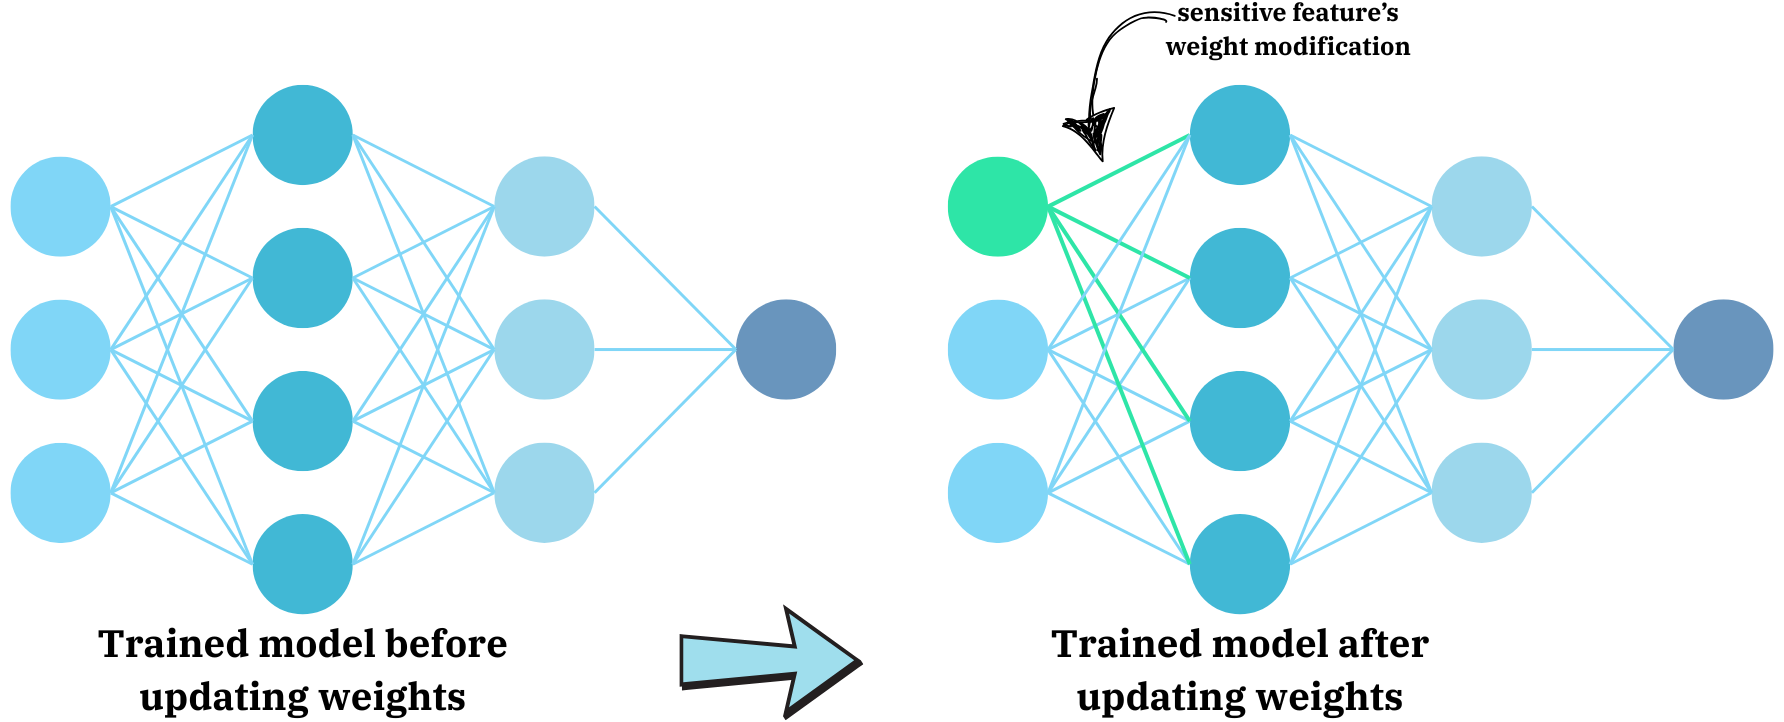
\includegraphics[width=.95\columnwidth]{figure/details_arc2.png}
  \caption{A detailed architecture of the DiRLU framework, where the teacher transfers knowledge to the student via knowledge distillation, integrated with post-hoc feature unlearning module for data privacy also reintroduce unlearned features for scalability}
  \label{fig1}
\end{figure}

%%%%%%%%%%%
\begin{table}[!ht]
    \centering
    \caption{Mathematical Symbols for Proposed Architecture}
    \renewcommand{\arraystretch}{0.9} % reduce row height
    \setlength{\tabcolsep}{6pt} % reduce column spacing
    \small % or \scriptsize
    \begin{tabular}{>{\raggedleft\arraybackslash}p{1.5cm} >{\raggedright\arraybackslash}p{10cm}}
        \toprule
        \textbf{Symbol} & \textbf{Description} \\
        \midrule
        \multicolumn{2}{l}{\textbf{Normalization}} \\
        \midrule
        $x$ & Original value of a feature\\
        $x_{\min}$ & Minimum value of a feature in the dataset \\
        $x_{\max}$ & Maximum value of a feature in the dataset \\
        $x'$ & Normalized value after Min-Max scaling \\
        \midrule
        \multicolumn{2}{l}{\textbf{Actor Network}} \\
        \midrule
        $\pi_\theta(a|s)$ & Policy function of the actor network with parameters $\theta$ \\
        $\theta$ & Parameters of the actor network \\
        $L_{\text{actor}}$ & Loss function for the actor network \\
        $A_t$ & Advantage function at time step $t$ \\
        $\alpha$ & Learning rate for the actor network \\
        $\nabla_\theta$ & Gradient with respect to actor parameters \\
        \midrule
        \multicolumn{2}{l}{\textbf{Critic Network}} \\
        \midrule
        $V_\phi(s_t)$ & Value function of the critic network for state $s_t$ \\
        $L_{\text{critic}}$ & Loss function for the critic network \\
        $R_t$ & Expected cumulative reward at time $t$ \\
        $r_t$ & Immediate reward at time step $t$ \\
        $\gamma$ & Discount factor in reinforcement learning \\
        $\beta$ & Learning rate for the critic network \\
        \midrule
        \multicolumn{2}{l}{\textbf{Knowledge Distillation}} \\
        \midrule
        $P_T(i)$ & Soft target probability from the teacher model for class $i$ \\
        $z_i$ & Logit (output) from the teacher model for class $i$ \\
        $T$ & Temperature parameter for softmax smoothing \\
        $P_S(i)$ & Student model’s predicted probability for class $i$ \\
        $y_i$ & Ground truth label for class $i$ \\
        $L_{\text{CE}}$ & Cross-entropy loss for true labels \\
        $L_{\text{KD}}$ & Distillation loss (KL divergence with soft targets) \\
        $L$ & Total loss function\\
        \midrule
        \multicolumn{2}{l}{\textbf{Evaluation}} \\
        \midrule
        $y_i$ & Ground truth label for class $i$ \\
        $\hat{y}_i$ & Predicted probability for class $i$ by the model  \\
        $n$ & The number of samples\\ 
        \bottomrule
    \end{tabular}
    \label{symbol_table}
\end{table}
%%%%%%%%%%%

\section{Data Description}
The BoT-IoT publicly available dataset was built in a real network environment in the Cyber Range Lab of the University of New South Wales (UNSW) Canberra \cite{data_des_1}. The environment was set in such a way that contained both normal and botnet network traffic. In the dataset, normal traffic is dominated by attack traffic. The dataset is heavily imbalanced, which reflects real-world cyberattack scenarios. They captured traffic using Wireshark, and the total size of pcap files is 69.3 GB, with more than 72 million records and 35 features. The Bot-IoT dataset includes different attacks such as DDoS, DoS, OS and Service Scan, Keylogging and Data exfiltration attacks, which are explained in Table-\ref{table_attackName}.

\begin{table}[!ht]
    \caption{Different cyber-attacks listed in the Bot-IoT dataset}
    \centering
    \renewcommand{\arraystretch}{0.9} % tighter row spacing
    \setlength{\tabcolsep}{4pt} % tighter column spacing
    \begin{tabular}{p{4.3cm} p{10cm}}
    \hline \hline
    \textbf{Attack Name} & \textbf{Description}\\ \hline
     
     Denial of Service (DoS) & An attempt to make a machine or network resource unavailable to its intended users\\ 

     Distributed Denial of Service (DDoS) & Multiple compromised systems attack a target, causing denial of service for users\\

     Reconnaissance & Activities aimed at gathering information about a network for planning future attacks\\

     Information Theft & Unauthorized access and retrieval of sensitive information\\

     Data Exfiltration & Unauthorized transfer of data from a computer or other device\\

     OS and Service Scan & This technique reveals systems and open service (HTTP, FTP, or SMTP) vulnerabilities\\

     Keylogging & This is a secret recording of a user’s keystrokes to capture sensitive information\\
     
     \hline \hline
    \end{tabular}
    \label{table_attackName}
\end{table}

In Table-\ref{table_data_des}, we listed all populated features (total 31) along with their description.

\begin{table}[!ht]
    \centering
    \caption{Feature description of the Bot-IoT dataset}
    \renewcommand{\arraystretch}{0.9} % tighter row spacing
    \setlength{\tabcolsep}{4pt} % tighter column spacing
    \begin{tabular}{l l}
    \hline
        \textbf{Feature Name} & \textbf{Feature Description} \\ \hline
        pkSeqID & Packet number \\
        stime & Packet capture start time \\ 
        flgs & Flow state flags seen in transactions \\
        flgs\_number & Numeric num. of flgs\\
        proto & Protocol used in the flow\\
        saddr & Source IP\\
        sport & Source port\\
        daddr & Destination IP\\
        dport & Destination port\\
        pkts & Total packet count\\
        bytes & Total bytes in the flow\\
        state & Packet state\\
        state\_number & Numeric num. of state\\
        ltime & Packet capture last time \\ 
        seq & Packet sequence number\\
        dur & Total duration\\
        min & Minimum duration of aggregated records\\
        max & Maximum duration of aggregated records\\
        mean & Average duration of total time\\
        stddev & Standard deviation of all records\\
        sum & Total duration of all records\\
        spkts & Source to destination packet count\\
        dpkts & Destination to source packet count\\
        sbytes & Byte count of source to destination packets\\
        dbytes & Byte count of destination to source packets\\
        rate & Packets per second in the flow\\
        srate & Packets per second from source to destination\\
        drate & Packets per second from destination to source\\
        attack & Label: 0 for Normal and 1 for Attack\\
        category & Network traffic category\\
        subcategory & Network traffic sub-category\\ \hline
    \end{tabular}
    \label{table_data_des}
\end{table}

\section{Data Pre-Processing}
Data pre-processing is required to ensure that the data fit properly into the proposed model as it standardizes, normalizes, and handles missing values. This alignment optimizes the model performance and accuracy by furnishing data with uniform, high-quality, and ideal inputs. Firstly, we have dropped the \textit{category and subcategory} column as we do not require them for classification. So, out of 35 features, we worked with 33 features; among them, we selected 32 features for further preprocessing. However, the column named \textit{attack} is used for classification.

\subsection{Feature Pruning}
To have a refined and clean dataset for training the model, we removed all missing or nan values. Some of the features didn't even have any values except nan. So, after removing all nan values, we got 27 columns and 15,000,000 rows. The completely empty features are \textit{smac, dmac, soui, doui, sco, }and\textit{ dco}.

\subsection{Label Encoding}
Label encoding is an essential technique for converting category input to numerical values, which makes it suitable for deep learning algorithms. For example,  we transformed the "attack" category, assigning the value 1 for attack and 0 for not attack. We utilized the \textit{LabelEncoder} function from the \textit{sklearn} library. This conversion allows the model to process the categorical data and use them for classification purposes.

\section{Data Split}
Splitting the dataset into a train, validation, and test subset is crucial for training, validating, and testing the model. We have taken 25\% of the total dataset, whereas previous state-of-the-art research has taken only 5\% \cite{n3}. We got 15,000,000 (Fifteen million) data points in 25\% of the whole dataset. We use a random splitting technique to split the dataset into three parts: training, validating, and testing. We took 70\% of data points for training, 10\% for validating \& tuning hyper-parameters, and another 20\% for testing the model. We randomly choose the 70:20:10 (train:test:validation) ratio for splitting the dataset. However, after splitting, we got 10,500,000 (Ten million five hundred thousand) data points for training the model, 1,500,000 (One million five hundred thousand) data points for tuning hyper-parameters \& validating the model, and 3,000,000 (Three million) data points for testing the model's performance.

\section{Data Augmentation}
We have taken 25\% data points from the BOT-IOT dataset, which gives us a total of 15,000,000 rows. Among those rows, we found attack rows 14,992,430 (Fourteen million, nine hundred ninety-two thousand, four hundred thirty) and the remaining 7,570 (Seven thousand five hundred seventy) non-attack rows. The dataset we have chosen for this research is highly imbalanced, and the ratio of attack vs non-attack is 98:2. So, to balance the dataset, we have used a technique called SMOTE.

SMOTE (Synthetic Minority Oversampling Technique) is an oversampling preprocessing technique used to address class imbalances in the dataset \cite{brandt2021comparative}. It generates synthetic data points by selecting a minority class and creating new data points along the line segments, attaching them to their closest neighbors. This method introduces diversity in the artificial samples, helping to create a non-biased dataset. SMOTE has been widely adopted in machine learning applications to enhance classification performance in imbalanced datasets \cite{chawla2002smote}.

\begin{figure}[htbp]
  \centering
  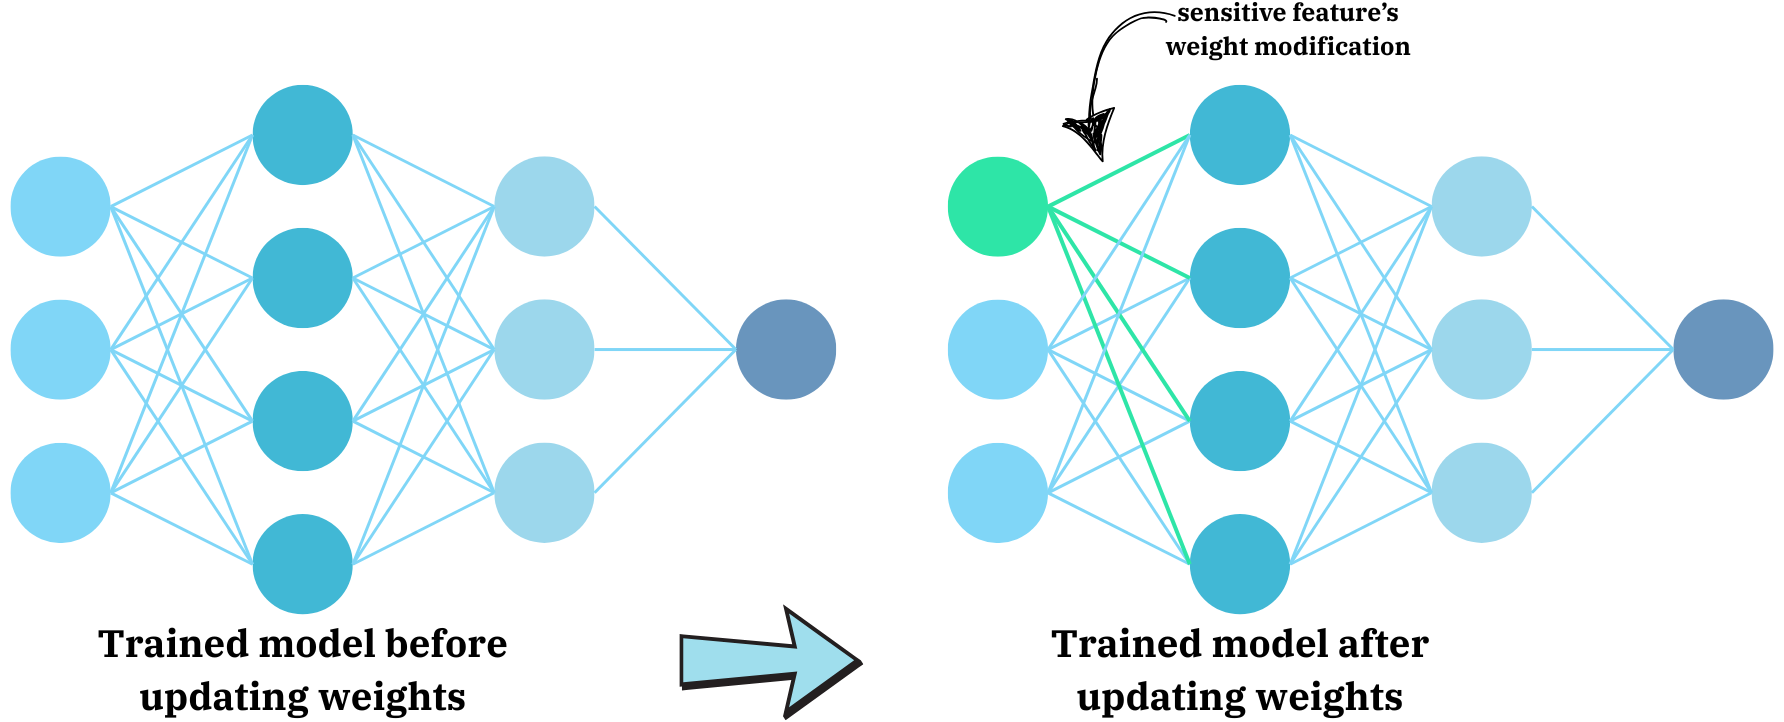
\includegraphics[width=0.65\columnwidth]{figure/fig-2.1.png}
  \caption{Comparison of before and after applying SMOTE}
  \label{fig2}
\end{figure}

After applying smote to the imbalance training dataset, we got 7,035,000 (Seven million thirty-five thousand) rows for the attack class (67\%) and another 3,465,000 (Three million four hundred sixty-five thousand) rows for the non-attack class (33\%), which makes the dataset balanced and non-biased. In Figure-\ref{fig2}, we have represented the ratio and effect of before \& after applying smote.

\section{Data Normalization}
Data normalization is a vital pre-processing technique required for scaling feature values. In the dataset, some feature values are large, and some are very small. Basically, it reshapes numerical values to fit into standard scale values. In this research, we applied deep learning techniques, so we used the Min-Max normalization technique to have values between 0 and 1. Recent studies have proved that Min-Max normalization can significantly improve the accuracy of deep learning models across various applications \cite{deepa2022epileptic}. The Min-Max function normalized the data using equation-\ref{eq:1}.

\begin{equation}\label{eq:1}
x' = \frac{x - x_{\text{min}}}{x_{\text{max}} - x_{\text{min}}}
\end{equation}

In equation-\ref{eq:1}, \(x\) is the original value, \(x_{\text{min}}\) is the minimum \& \(x_{\text{max}}\) is the maximum value in the dataset, and \(x'\) is the normalized value.

\section{Reinforcement Learning}
Reinforcement learning is a type of machine learning where the model learns by interacting with its environment and receiving rewards or penalties for each of its actions, similar to trial and error \cite{RF_IBM}. Unlike traditional deep learning, it does not rely on labeled data but improves through feedback. It is beneficial for solving complex problems like IoT Security \cite{uprety2020reinforcement}.

We have used the actor-critic model because of its enhanced stability compared to traditional reinforcement learning approaches by combining policy optimization with value estimation. In the Fig-\ref{RF_arc}, we represented a simple architecture of the actor-critic model. The actor-critic framework operates through two interconnected neural networks that collaborate to optimize decision-making processes. The actor-network functions as a policy generator, determining which actions to execute based on current states. In contrast, the critic network serves as an evaluator, assessing the quality and long-term value of the actor's chosen actions. During training, the actor adjusts its policy parameters using feedback signals provided by the critic, which simultaneously refines its value estimations based on observed rewards and feedback. This mechanism creates a balanced learning environment by exploring new strategies. The temporal difference error, calculated as the dissimilarity between predicted and actual rewards, is the primary learning signal that guides both networks toward optimal performance \cite{actor_critic_tensorflow}. The actor updates its policy through gradient ascent on expected rewards, while the critic minimizes prediction errors through standard value function approximation techniques. This iterative process continues until convergence, resulting in a robust policy that maximizes cumulative rewards while maintaining stable learning dynamics throughout the training process.

\begin{figure}[htbp]
  \centering
  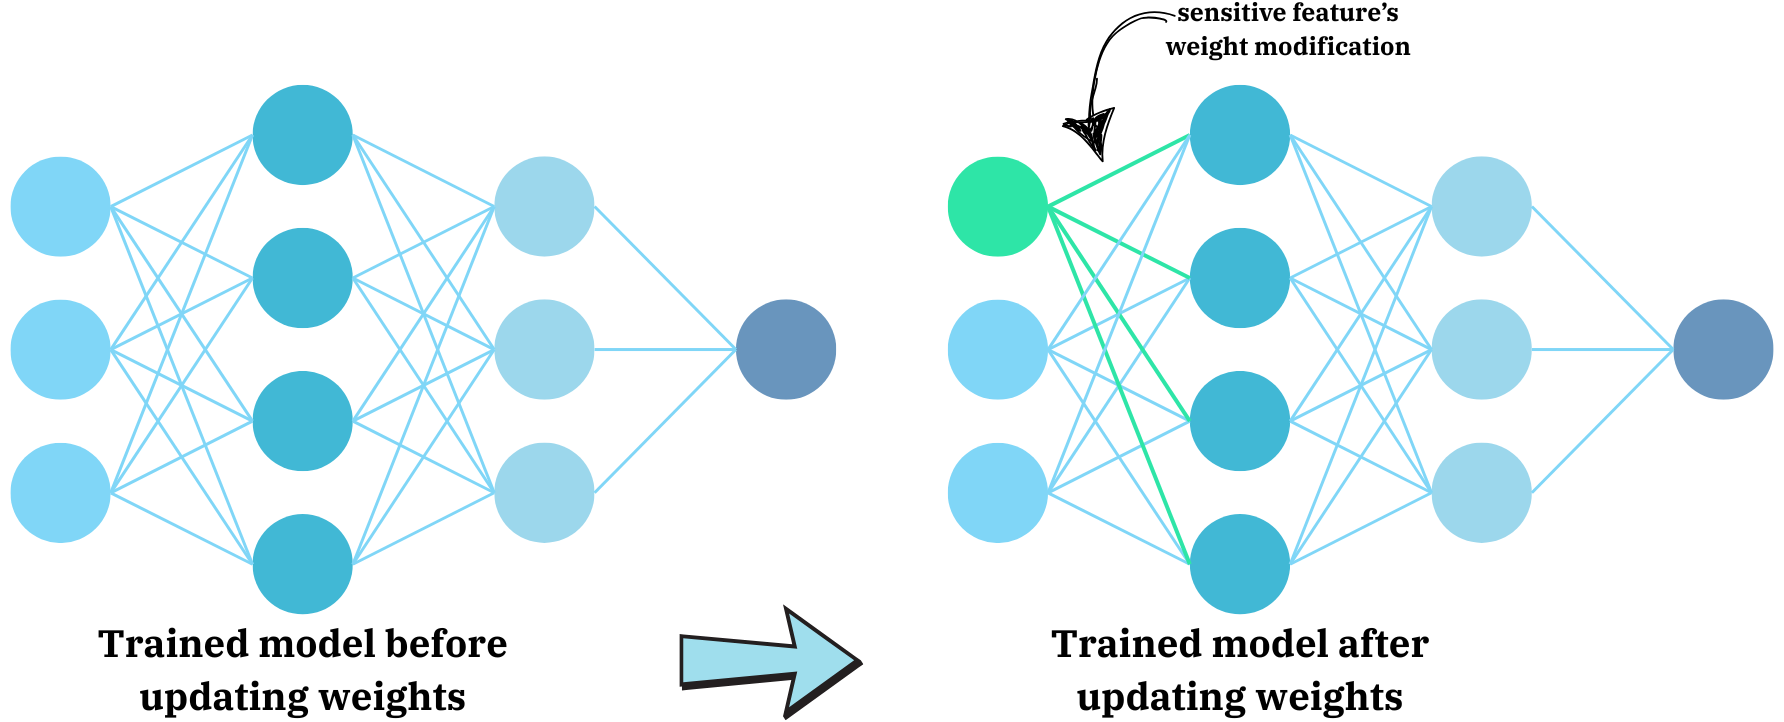
\includegraphics[width=0.60\columnwidth]{figure/RF_arc1.png}
  \caption{Actor-Critic model architecture}
  \label{RF_arc}
\end{figure}

From equations \ref{policy_function}-\ref{critic_update}, we have described the mathematical formulas of the actor-critic model, including both forward propagation and backpropagation update rules.

\begin{equation}\label{policy_function}
\pi_\theta(a|s) = P(a|s; \theta)
\end{equation}
In equation-\ref{policy_function} is Actor Policy Function is shown where the probability of taking action $a$ in state $s$, and $\theta$ denotes the actor network parameters.

\begin{equation}\label{actor_loss}
L_{actor} = -\mathbb{E}[\log \pi_\theta(a_t|s_t) \cdot A_t]
\end{equation}
In equation-\ref{actor_loss} shows the actor loss function, where $A_t$ is the advantage function and $\mathbb{E}[\cdot]$ represents the expected value operator.

\begin{equation}\label{value_function}
V_\phi(s_t) = \mathbb{E}[R_t|s_t]
\end{equation}
In equation-\ref{value_function} shows Critic Value Function where critic parameters is $\phi$, and $R_t$ denotes the expected cumulative reward.

\begin{equation}\label{critic_loss}
L_{critic} = \mathbb{E}[(r_t + \gamma V_\phi(s_{t+1}) - V_\phi(s_t))^2]
\end{equation}
In equation-\ref{critic_loss}, the critic loss function is shown, where $V_\phi(s_t)$ is the state value function, $\gamma$ represents the discount factor, and $r_t$ is the immediate reward at time step $t$.

\begin{equation}\label{actor_update}
\theta \leftarrow \theta + \alpha \nabla_\theta \log \pi_\theta(a_t|s_t) \cdot A_t
\end{equation}
In equation-\ref{actor_update} presents the actor parameter update rule, where $\alpha$ is the learning rate and $\nabla_\theta$ represents the gradient with respect to actor parameters.

\begin{equation}\label{critic_update}
\phi \leftarrow \phi - \beta \nabla_\phi L_{critic}
\end{equation}
In equation-\ref{critic_update}, the critic parameter update is shown, where $\beta$ is the critic learning rate and $\nabla_\phi$ denotes the gradient with respect to critic parameters.

We used actor-critic reinforcement learning in a teacher-student framework for knowledge distillation. In this design, the teacher model has two outputs: the actor makes binary classification decisions using a sigmoid function, and the critic provides continuous value estimates with a linear function. We added an attention mechanism that learns to focus on all the input features with an entropy regularization. We also implemented shared hidden layers, L2 and dropout regularization for better generalization. We use weighted loss functions to handle class imbalance so that underrepresented classes get fair attention during training. Overall, the model jointly optimizes three goals: accurate classification by the actor, precise value estimation by the critic, and balanced attention. This multi-objective setup helps the teacher learn rich representations, which are then passed on to the student model for better learning.

\section{Knowledge Distillation}
Knowledge Distillation (KD) is a model compression technique where a large, complex teacher model transfers its knowledge to a smaller, more efficient student model without significant loss in performance. In this method, the teacher model is initially trained on a dataset, and its output, such as soft probabilities (logits) or intermediate feature representations, is used to assist the student model's training. The student model is optimized using a distillation loss function, which combines standard loss (cross-entropy) with a term encouraging the student to mimic the teacher's outputs. The benefit of the KD is that it reduces the size of networks while maintaining high accuracy and faster inference, making it appropriate for deployment on resource-constrained devices such as mobile phones and edge computing platforms. This technique has been widely adopted in security applications, improving the robustness of AI models against adversarial attacks while maintaining efficiency \cite{gou2021knowledge}. We have used KD to classify malware and begin traffic with low resources. In Fig-\ref{fig4}, we have included an architecture diagram of the knowledge distillation model.

\begin{figure}[htbp]
  \centering
  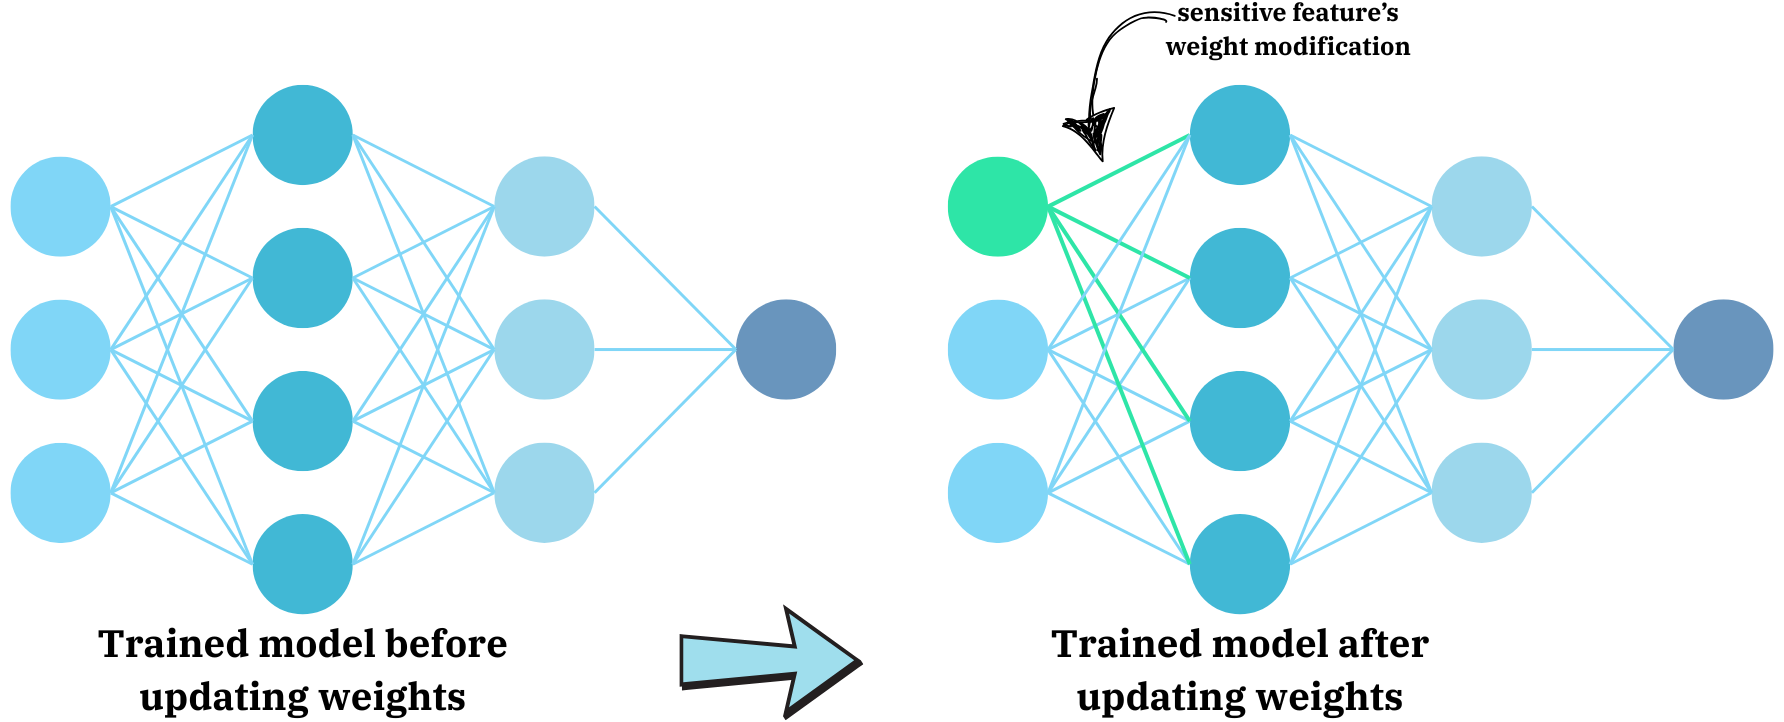
\includegraphics[width=0.65\columnwidth]{figure/fig-4.png}
  \caption{Architecture of knowledge distillation (KD) framework}
  \label{fig4}
\end{figure}

\subsection{Teacher Model}\label{Teacher Model}
We implemented a teacher model within a Knowledge Distillation (KD) framework, where a larger Actor-Critic model transfers its knowledge to a smaller one (student model). The teacher model learns to map input data to output probabilities, which are then used to transfer knowledge to a smaller one. The teacher model produces soft targets $P_T$ by applying a temperature-scaled softmax function to the logits:

\begin{equation}\label{eq:2}
P_T(i) = \frac{\exp(z_i / T)}{\sum_{j} \exp(z_j / T)}
\end{equation}

In equation-\ref{eq:2}, $z_i$ is the logit (output) from the teacher model and 
$T$ is the temperature hyperparameter, which controls the smoothness of the probability distribution. Higher $T$ produces smoother probability distributions.

The teacher model is an attention-enhanced actor-critic architecture. It includes a feature-level attention mechanism that learns from all the individual input features. The attended representation is concatenated with the original input and passed through three shared dense layers with ReLU activation and L2 regularization. The actor's head generates probability scores using a sigmoid activation, while the critic's head estimates value functions using a linear activation. An additional entropy penalty regularizes the attention weights to prevent overly confident focus on a few features. Class weights are dynamically computed and incorporated into the custom binary cross-entropy loss function to address class imbalance. Furthermore, the model uses early stopping on validation accuracy to avoid overfitting and restore the best-performing weights. Training continues until early stopping is triggered, typically within 25–30 epochs. Table-\ref{table_4} provides a complete list of the hyperparameters and their corresponding values used to improve the teacher model's performance.

\begin{table}[!ht]
    \centering
    \caption{Hyperparameters used in teacher model}
    \renewcommand{\arraystretch}{0.9} % tighter row spacing
    \setlength{\tabcolsep}{4pt} % tighter column spacing
    \begin{tabularx}{0.9\columnwidth}{l X} % U
    \hline
        \textbf{Hyperparameter} & \textbf{Value} \\ 
            \hline
            Model & Actor-Critic \\
            Number of Hidden Layers & 3 \\
            Activation Function (Hidden Layers) & ReLU \\
            Activation Function (Actor Output) & Sigmoid \\
            Activation Function (Critic Output) & Linear \\
            Regularization & L2 \& Entropy Penalty\\
            Actor Loss Function & Weighted BSE\\
            Critic Loss Function & MSE\\
            Optimizer & Adam \\
            Epoch Number & Early stopping (max 30)\\
            Batch Size & 512 \\
            Evaluation Metric & Accuracy \& F1 Score \\
            \hline
    \end{tabularx}
    \label{table_4}
\end{table}

To make predictions, probability scores from the actor's head are binarized using a 0.8 threshold, and the F1 score is calculated to evaluate classification performance. This trained teacher model is the foundation for knowledge transfer, guiding the development of a smaller, more efficient student model with similar decision boundaries and attention-driven behaviour.

\subsection{Student Model}\label{Student Model}
A student model is a smaller, more efficient Actor-Critic model trained to replicate the behaviour of a larger and more complex teacher model. It learns using the teacher's softened predictions, allowing it to perform well while being lightweight and faster. With appropriate distillation techniques, student models can accurately mimic the behaviour of the teacher model while drastically reducing the model size and computational complexity, making them ideal for real-time applications in mobile and edge computing \cite{chen2022improved}. The student model mimics the teacher's behavior by optimizing a total loss that combines standard cross-entropy (for true labels) and distillation loss (KL divergence with the teacher's soft targets).\\

The Cross-Entropy Loss for true labels $(L_{\text{CE}})$,

\begin{equation}\label{eq:3}
L_{\text{CE}} = -\sum_{i} y_i \log P_S(i)
\end{equation}

In equation-\ref{eq:3}, $ y_i$ is the ground truth label and $P_S(i)$ is the student model's predicted probability.\\

Distillation Loss (KL divergence with soft targets) $(L_{\text{KD}})$,

\begin{equation}\label{eq:4}
L_{\text{KD}} = T^2 \sum_{i} P_T(i) \log \frac{P_T(i)}{P_S(i)}
\end{equation}

In equation-\ref{eq:4}, $T$ is temperature parameter which controls the smoothness of the probability distribution, $P_T(i)$ is probability output from the teacher model of class $i$ and $P_S(i)$ is probability output from the student model of class $i$.\\

The total loss function $(L)$,

\begin{equation}\label{eq:5}
L = \alpha L_{\text{CE}} + (1 - \alpha) L_{\text{KD}}
\end{equation}

In equation-\ref{eq:5}, $\alpha$ is a weighting factor that balances the cross-entropy loss $L_{\text{CE}}$ and the distillation loss $L_{\text{KD}}$.\\

In this research, the student model consists of a smaller actor-critic model. This student model is smaller and faster than the teacher model. The actor helps predicts the final class (benign or attack), and the critic, which gives a value or score to help guide learning.

We use an attention mechanism to make the model focus on all the input features. These attention-weighted inputs are combined with the original input and passed through two hidden layers. Each layer uses the ReLU activation function, and we apply L2 regularization to reduce overfitting. The final part of the model has two outputs: the actor output uses a sigmoid function for classification, and the critic output uses a linear function to estimate value. We also apply an entropy penalty on the attention weights to ensure the model doesn’t focus too much on only a few features. We train the model using the Adam optimizer with a batch size 32. The actor output is trained with a custom loss function that combines two types of loss: binary cross-entropy, which checks how well the predictions match the actual labels, and KL divergence, which helps the student learn from the soft outputs of the teacher model. We use a temperature value of 2.0 to smooth the teacher’s predictions and an alpha value 0.5 to balance the two losses. For the critic output, we use mean squared error with class weights to handle imbalance in the data. We also include the entropy penalty in the total loss to balance the attention distribution. We use early stopping based on validation accuracy to avoid overfitting, which stops training when the model stops improving. Table-\ref{table_5} provides the list of the hyperparameters and their corresponding values used to improve the student model’s performance.

\begin{table}[!ht]
    \centering
    \renewcommand{\arraystretch}{0.9} % tighter row spacing
    \setlength{\tabcolsep}{4pt} % tighter column spacing
    \caption{Hyperparameters used in student model}
    \begin{tabularx}{0.9\columnwidth}{l X} % Use 'X' for the second column to auto-adjust width
    \hline
        \textbf{Hyperparameter} & \textbf{Value} \\ 
        \hline
        Model & Actor-Critic \\
        Number of Hidden Layers & 2 \\
        Activation Function (Hidden Layers) & ReLU \\
        Activation Function (Actor Output) & Sigmoid \\
        Activation Function (Critic Output) & Linear \\
        Regularization & L2 \& Entropy Penalty\\
        Actor Loss Function & Distillation Loss (CE+KL)\\
        Critic Loss Function & Weighted MSE\\
        Temperature & 2.0 \\
        Alpha & 0.5 \\
        Optimizer & Adam \\
        Epoch Number & Early stopping (max 30)\\
        Batch Size & 512 \\
        Evaluation Metric & Accuracy \& F1 Score \\
        \hline
    \end{tabularx}
    \label{table_5}
\end{table}

%%%%%%%%%%%%%CHANGE KORTE HOBE UPTO THIS POINT%%%%%%%%%%%%%%

\section{Un-learning}
Feature unlearning is a technique designed to remove the influence of specific features from a trained model, ensuring that once removed, those features no longer affect the model’s outputs.
The Price of Forgetting \cite{PriceOfForgetting} introduced an economic approach by offering payments to users for keeping their data, helping servers reduce costs while still respecting user privacy. While our approach plays an important role in meeting privacy regulations, mitigating security risks (such as eliminating data), and enabling efficient model updates without the need for full retraining. Key benefits include regulatory compliance by securely removing sensitive data, cost and time savings from avoiding comprehensive retraining, and greater transparency and trust in AI systems. Recent developments in feature unlearning have introduced methods such as data pruning and selective retraining, which allow models to effectively erase the impact of targeted features while preserving overall performance \cite{zhang2023machine}. In practice, this balance of privacy, efficiency, and model reliability is critical for real-world applications.

The post hoc weight modification technique is used to "forget" sensitive data/features for data security. Instead of retraining the whole model, this technique sets zero weight in the first layer of the specific feature. Post hoc weight modification (PHWM) allows the model to forget specific features by modifying a single weight in the network without costly and time-consuming retraining \cite{hakemi2025post}. In Fig-\ref{PHWM}, we illustrate the process of unlearning.

\begin{figure}[htbp]
  \centering
  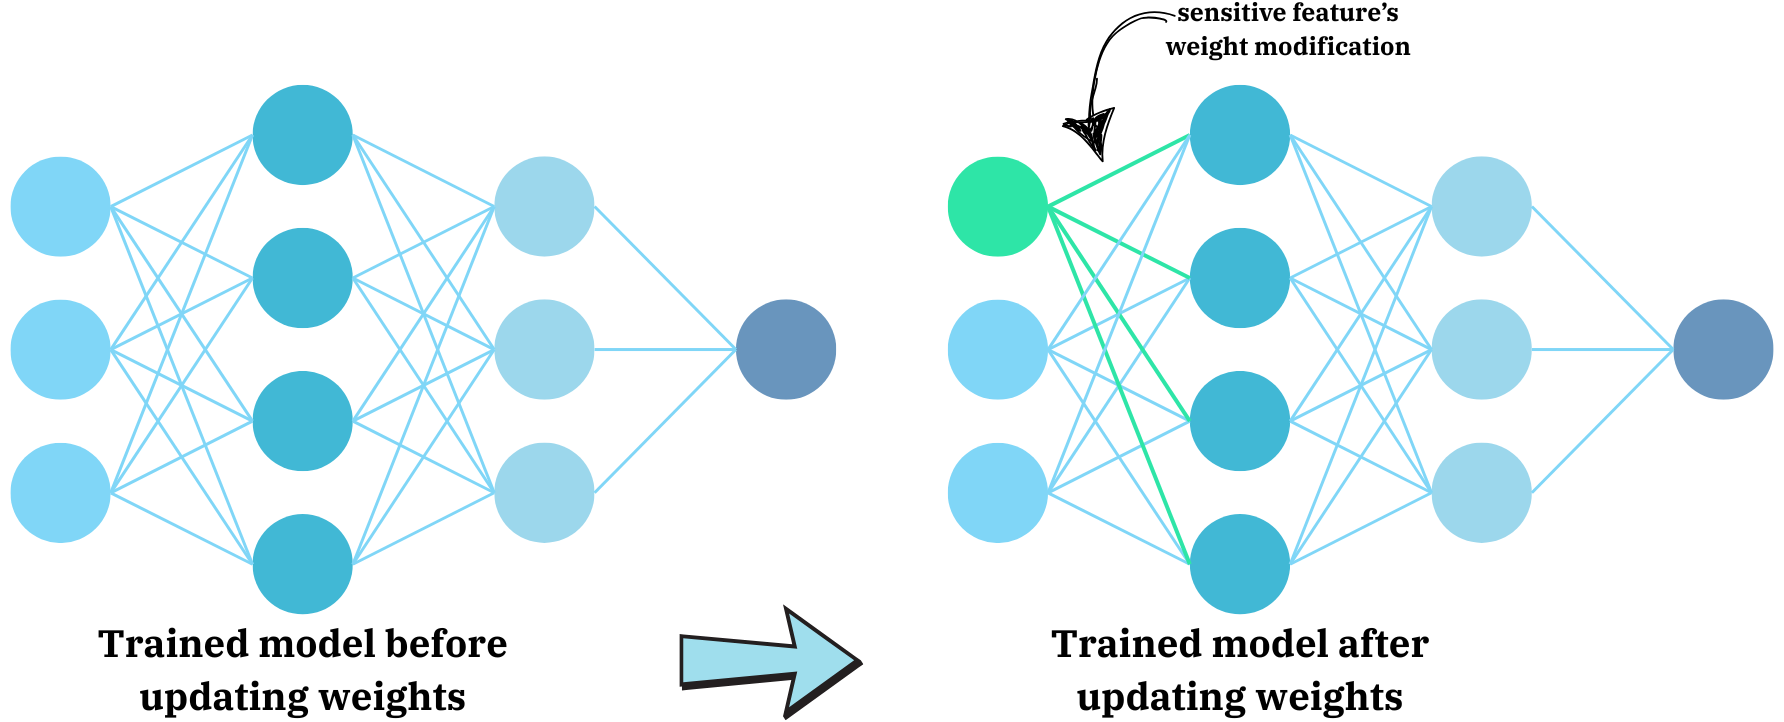
\includegraphics[width=0.95\columnwidth]{figure/deep unlearn.png}
  \caption{Architecture of feature unlearning process}
  \label{PHWM}
\end{figure}

\subsection{Teacher Unlearn}
The procedure of teacher unlearning involves selectively dismissing the second top feature from the dataset that has the most impact on the teacher model. We have used XAI to identify the feature. In this experiment, we have found the second top feature, '\textit{flgs}', for removal from the pre-trained teacher. We removed the feature from the input datasets to ensure the model unlearned them. We also set their corresponding weights in the first layer of the network to zero, preventing them from influencing predictions. After modifying the weight matrix, we reloaded it into the model to ensure the feature was no longer used. To measure the impact of these changes, we re-evaluated the model using accuracy and F1-score. This approach helps improve model interpretability by removing redundant or sensitive features and keeping computations efficient. The approach ensures that the model no longer depends on the removed features, enforcing unlearning at both the data and model levels.

\subsection{Student Unlearn}
The process of student unlearning involves carefully removing the second most influential feature from the dataset that affects the student model. We used XAI to specify the features; in this case, the feature was 'flgs'. The feature was removed from the input datasets to ensure the student model no longer learned or made predictions using them. We set the corresponding weights of the feature in the network's first layer to zero, ensuring the model couldn't rely on them for predictions. After making these changes to the weight matrix, the feature was refilled into the student model to confirm that they were no longer in use. To understand how this influenced the model, we re-evaluated it using accuracy and F1-score. This approach improves the model's interpretability by removing unnecessary or sensitive features while maintaining efficient computations.


\section{Explainable Artificial Intelligence (XAI)}
Explainable AI (XAI) in machine learning and deep learning focuses on making model decisions more transparent and easier to understand. It demonstrates how models arrive at their predictions, which helps build trust and ensures fairness. XAI is also valuable for assessing feature importance by showing how different factors influence model outcomes, an essential step for tuning models and improving performance. By improving interpretability, XAI supports accountability and strengthens the reliability of AI systems. Common approaches include local and global interpretability methods such as SHAP and LIME, which provide insights into both individual predictions and overall model behavior, making it easier to detect biases or errors in decision-making \cite{ribeiro2016should}. Recent work has also applied XAI to anomaly detection in NFV systems, where masked autoencoders are combined with explainability techniques to enhance interpretability and support effective fault localization \cite{AnomalyNFV}.

We used LIME (Local Interpretable Model-agnostic Explanations) to understand how the model makes decisions. LIME explains predictions by generating minor variations around a given data point and analyzing how the model responds. LIME has been applied in diverse machine learning tasks, enhancing model transparency and helping researchers identify potential biases or errors in model predictions \cite{gilpin2018explaining}. A single test instance was randomly chosen, and LIME ranked the top 12 features that influenced the model's conclusion. The explanation mode was set to classification, and discretization was turned off to retain continuous feature representations. The Results were visualized interactively using show\_in\_notebook(). Using LIME, we gained valuable insights into which features played a key role in the model's classification.

\section{Model Evaluation}
In this research, we tested the model's performance using various commonly used metrics, such as accuracy, F1 score, and loss.

Regardless of class, accuracy determines the overall accuracy of the model's predictions and evaluates its performance.

\begin{equation}\label{eq:6}
\textit{Accuracy} = \frac{\textit{TP} + \textit{TN}}{\textit{TP} + \textit{TN} + \textit{FP} + \textit{FN}}
\end{equation}

Precision measures the percentage of the model's predictions that are correct, and recall measures the percentage of relevant data points that the model correctly identified. The mean of precision and recall is the F1 score.

\begin{equation}\label{eq:7}
\textit{Precision} = \frac{\textit{TP}}{\textit{TP} + \textit{FP}}
\end{equation}

\begin{equation}\label{eq:8}
\textit{Recall} = \frac{\textit{TP}}{\textit{TP} + \textit{FN}}
\end{equation}

\begin{equation}\label{eq:9}
\textit{F1 score} = \frac{\textit{2*Precision*Recall}}{\textit{Precision} + \textit{Recall}}
\end{equation}

In equations \ref{eq:6}-\ref{eq:9}, $TP$ denotes true positives, $TN$ denotes
true negatives, $FP$ denotes false positives, and $FN$ denotes
false negatives.

Another evaluation metric, Binary Cross-Entropy ($BCE$) is a loss function used in this paper for binary classification. It measures the difference between accurate labels ($y$) and predicted probabilities ($\hat{y}$). It penalizes inaccurate predictions more when predictions are confident but wrong.


\begin{equation}\label{eq:10}
\text{BCE} = - \frac{1}{n} \sum_{i=1}^{n} \left[ y_i \log(\hat{y}_i) + (1 - y_i) \log(1 - \hat{y}_i) \right]
\end{equation}

In the equation \ref{eq:10}, $y_i$ is the actual label, $\hat{y}_i$ is the predicted probability, and $n$ is the number of samples.

\section{Proposed Algorithm}
In algorithm-\ref{pseudocode}, we explain the pseudocode for the proposed model's architecture in detail. We built the model using Python (v3.12) and different libraries, such as tensorflow, pandas, lime, matplotlib, etc., on Visual Studio Code IDE.

\begin{algorithm*}[!htb]
\caption{Pseudocode of DiRLU}
% --- compact settings ---
\algrenewcommand\algorithmicindent{0.6em}
\algrenewcommand\alglinenumber[1]{\footnotesize #1}
\small % or \scriptsize for even tighter
\resizebox{0.99\linewidth}{!}{%
\begin{minipage}{\linewidth}
\begin{algorithmic}[1]

\Function{Preprocess}{df}
  \State $df_c \gets \textproc{Clean}(df)$; $df_b \gets \textproc{ApplySmote}(df_c)$; $df_{tr}, df_{val}, df_{te} \gets \textproc{Split}(df_b)$
  \State \Return $df_{tr}, df_{val}, df_{te}$
\EndFunction

\vspace{0.4em}

\Function{TrainA2CTeacher}{df\_train}
  \State $teacher \gets \textproc{A2C()}$;\; $w \gets \textproc{CompClsWeights}(df\_train)$
  \While{NOT \textproc{Converged}(teacher, EarlyStop)}
    \State $(x,y) \gets \textproc{Sample}(df\_train)$
    \State $L \gets \textproc{WeightedBCE}(actor(x), y, cls\_weights)+\textproc{MSE}(critic(x), y)$
    \Statex \hspace{1.5cm}$+ \lambda_{attn}\cdot \textproc{Entropy}(attention)$
    \State \textproc{UpdateA2C}$(teacher,\nabla L,\text{Adam})$
  \EndWhile
  \State \Return $teacher$
\EndFunction

\vspace{0.4em}

\Function{FeatureUnlearn}{model, forgetFeat}
  \State $(W_u, b_u) \gets model.\textproc{GetWeights}(\texttt{first\_dense},\textproc{Index}(forgetFeat))$
  \State $W_v \gets 0.0$; $b_v \gets 0.0$
  \State $model \gets model.\textproc{UpdateWeights}(\texttt{first\_dense},\textproc{Index}(forgetFeat), W_v, b_v)$
  \State \Return model
\EndFunction

\vspace{0.4em}

\Function{DistillToStudent}{teacher, df\_train, T}
  \State $student \gets \textproc{A2C()}$; $cls\_weights \gets \textproc{ComClsWeights}(df\_train)$
  \State $t\_probs \gets \textproc{Softmax}(teacher(df\_train)/T)$
  \While{NOT \textproc{Converged}(student, EarlyStop)}
    \State $(x, y) \gets \textproc{Sample}(df\_train)$
    \State $L \gets \alpha \cdot \textproc{CE}(student(x), y) + (1-\alpha) \cdot T^2 \cdot \textproc{KL}(student(x)/T,\ t\_probs)$
    \Statex \hspace{1.5cm}$+ \textproc{MSE}(critic(x), y) + \lambda_{attn} \cdot \textproc{Entropy}(attention)$
    \State \textproc{Step}(student, $\nabla L$, Adam)
  \EndWhile
  \State \Return $student$
\EndFunction

\vspace{0.4em}

\Function{RestoreFeatures}{model, forgetFeat}
  \State $(W_v, b_v) \gets \textproc{SavedWeightsBiases}(\texttt{first\_dense},\textproc{Index}(forgetFeat))$
  \State $model \gets model.\textproc{UpdateWeights}(\texttt{first\_dense},\textproc{Index}(forgetFeat), W_v, b_v)$
  \State \Return model
\EndFunction

\vspace{0.4em}

\State $df_{tr}, df_{val}, df_{te} \gets \Call{Preprocess}{df}; teacher \gets \Call{TrainA2CTeacher}{df_{tr}}$
\State $student \gets \Call{DistillToStudent}{teacher,\ df_{tr},\ T}$

\vspace{0.2em}

\State $base\_models (\mathcal{B}) \gets [teacher,\ student]$
\State $unlearn\_models (\mathcal{UL}) \gets [\,]$
\State $restore\_models (\mathcal{RE}) \gets [\,]$

\vspace{0.2em}

\ForAll{$m \in base\_models$}
  \State $unlearn\_models \gets \Call{FeatureUnlearn}{m,\ df_{fg}}$
\EndFor

\vspace{0.2em}

\ForAll{$m\_ul \in unlearn\_models$}
  \State $restore\_models \gets \Call{RestoreFeatures}{m\_ul,\ df_{fg}}$
\EndFor

\vspace{0.2em}

\State $all\_models \gets\mathcal{B} \cup \mathcal{UL} \cup \mathcal{RE}$

\ForAll{$x \in df_{te}$}
  \ForAll{$m \in all\_models$}
    \State $\hat{y} \gets \textproc{Predict}(m,\ x)$
    \State $\Call{ExplainWithLIME}{\hat{y}}$
  \EndFor
\EndFor
\State $\textproc{CompareResults}(all\_models)$

\end{algorithmic}
\end{minipage}}
\label{pseudocode}
\end{algorithm*}

To conduct the research, a high-performance workstation was configured with 64GB of RAM, a 3.40GHz processor, and an NVIDIA 12GB GPU running Windows 11. This setup ensured optimal processing and memory capacity for data-intensive tasks.

\chapter{Result and Analysis}\label{result_and_analysis}
This chapter presents a comprehensive and rigorous evaluation of the Continuous Latent Autoencoder (CLAE) trained for Bengali speech representation learning. The primary objective of this chapter is to thoroughly dissect the model's behavior during pre-training and evaluate its learned representations. We detail the complex training dynamics, analyze the structural integrity of the latent space representations, and inspect the signal reconstruction behaviors under various acoustic conditions. Furthermore, we present critical ablation studies that validate the necessity of our composite loss function. Finally, a comparative analysis against established state-of-the-art models is conducted to demonstrate the efficacy, parameter efficiency, and competitive downstream performance of our proposed approach.

\section{Pre-training Convergence and Component Loss Analysis}

The foundation of our self-supervised learning strategy is a highly specialized composite loss objective, mathematically defined as $L = 1.0 L_{mel} + 0.3 L_{JEPA} + 0.7 L_{VISReg}$. The integration of these three independent, yet complementary, loss components ensures that the model can effectively compress continuous audio streams into a low-dimensional space without suffering from representation collapse—a notoriously difficult challenge in continuous autoencoder architectures. By balancing reconstruction fidelity with structural regularization, the model learns phonetic abstractions rather than merely memorizing acoustic noise.

Figure \ref{fig:training_loss} illustrates the total training trajectory over an extended pre-training period of 170,700 steps. The total loss exhibited remarkably stable convergence, initiating at an expectedly high value of approximately 5.45 during the first 50 steps. As the convolutional feature extractor and the transformer-based decoder synchronized, the loss decayed rapidly, eventually stabilizing at 1.34 near step 167,500. This smooth asymptotic decline, punctuated only by minor fluctuations during learning rate adjustments, indicates that the model avoided catastrophic forgetting and successfully localized a robust global minimum in the optimization landscape.

\begin{figure}[htbp]
    \centering
    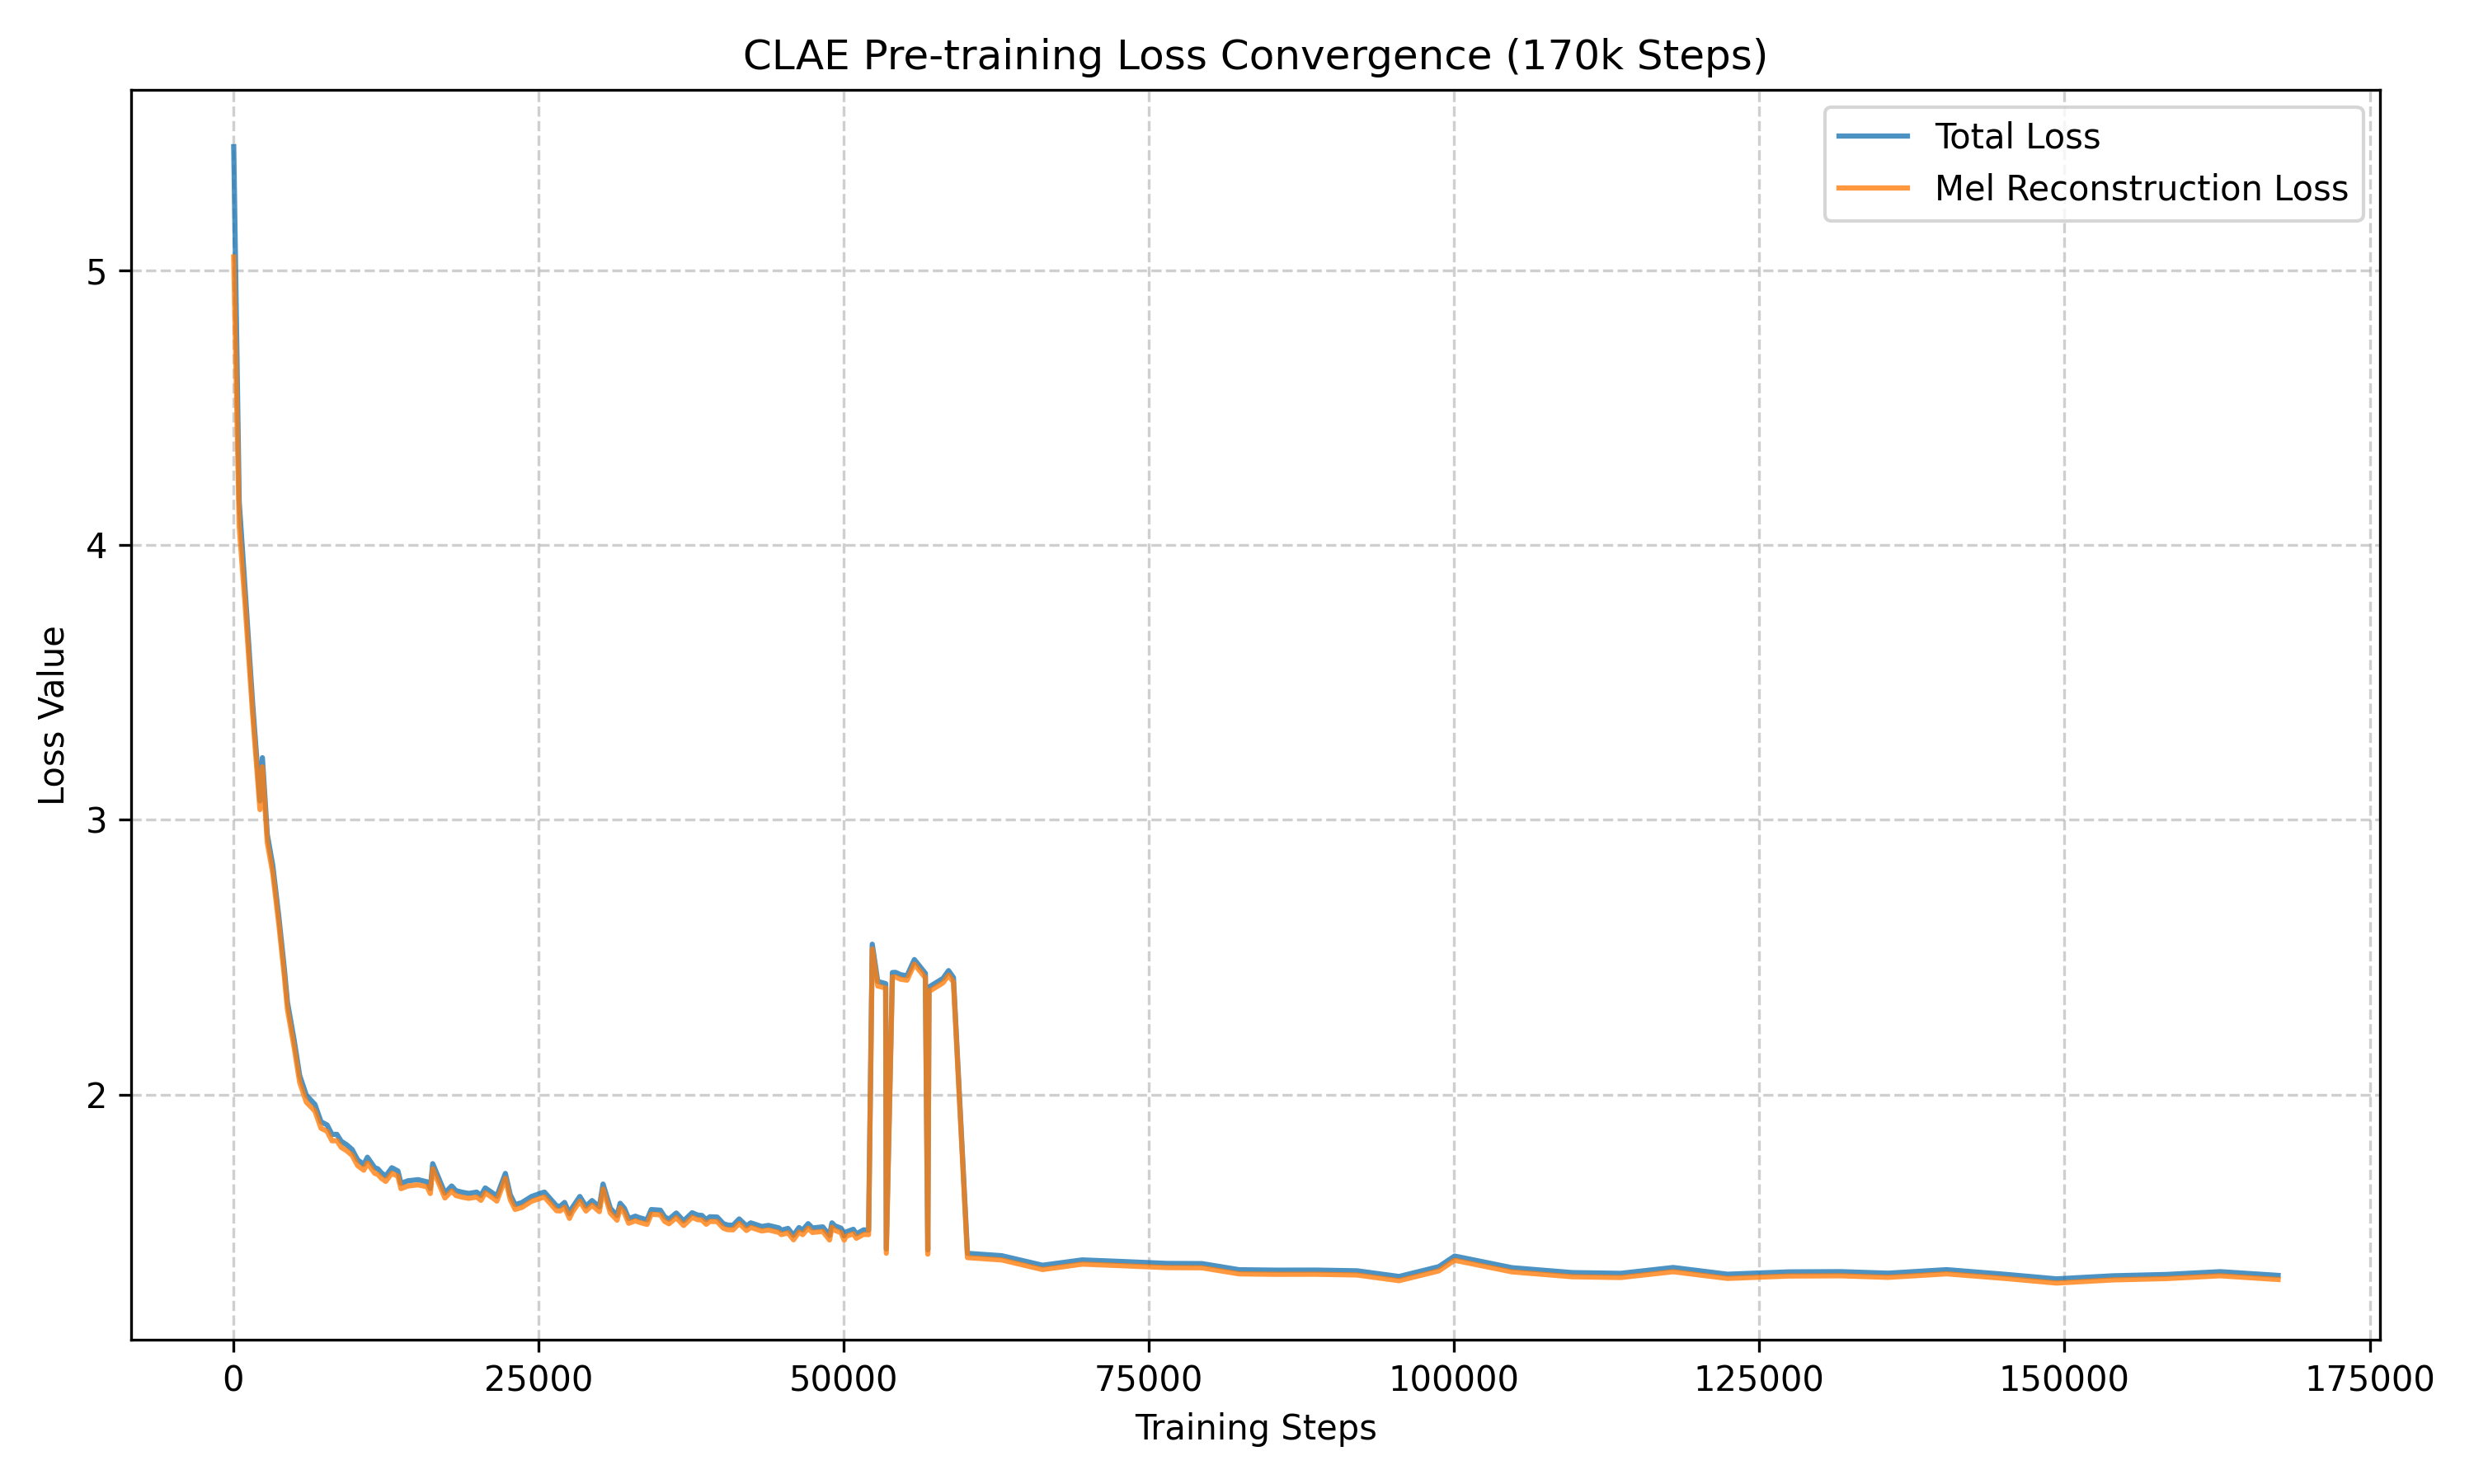
\includegraphics[width=0.85\textwidth]{figure/training_loss.png}
    \caption{Pre-training loss convergence of the CLAE model over 170k steps, depicting the tight correlation between Total Loss and the primary Mel Reconstruction Loss.}
    \label{fig:training_loss}
\end{figure}

Beyond the primary Mel Reconstruction Loss ($L_{mel}$), the self-supervised regularization components played a paramount role in shaping the topological structure of the feature space. Figure \ref{fig:component_loss} visualizes the isolated dynamics of $L_{JEPA}$ (which explicitly enforces contextual consistency over temporal sequences) and $L_{VISReg}$ (which enforces dimensional decorrelation and variance maximization within the embeddings). The steady, monotonic decline of $L_{VISReg}$ is particularly noteworthy; it mathematically confirms that the model successfully learned a distributed representation, utilizing the full bandwidth of the embedding vector rather than clustering all phonetic information into a few redundant, dominant dimensions.

\begin{figure}[htbp]
    \centering
    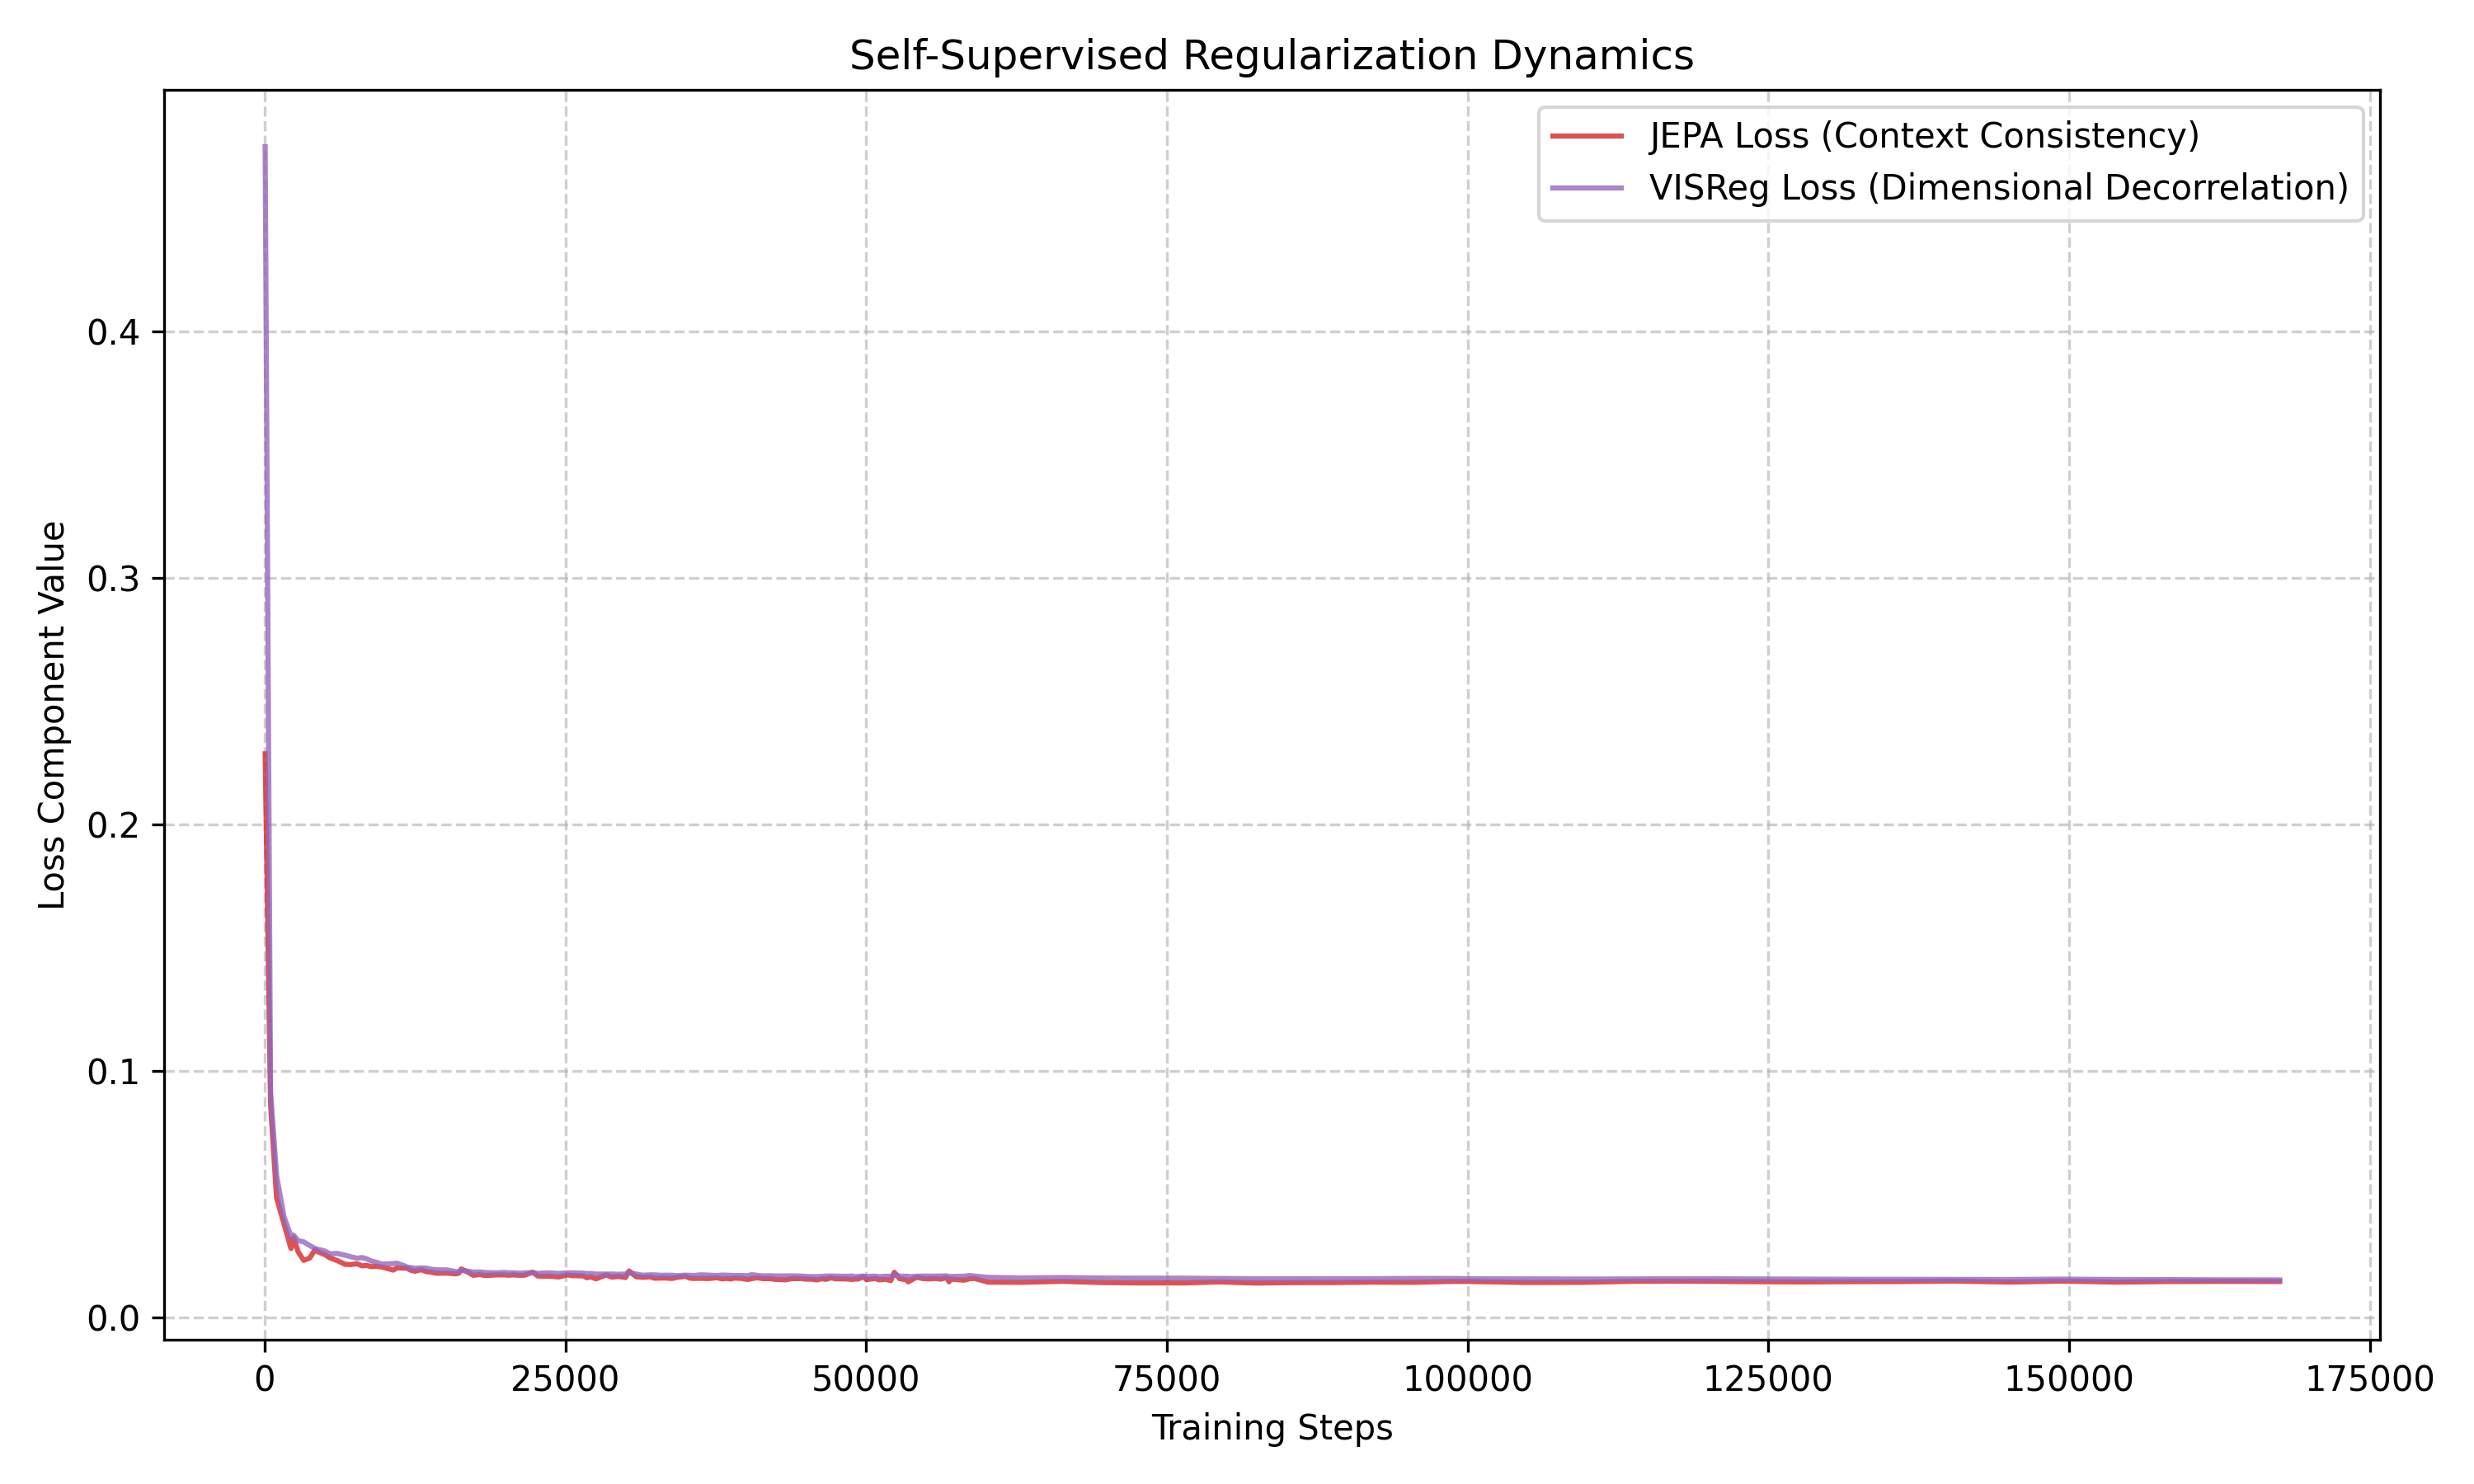
\includegraphics[width=0.85\textwidth]{figure/component_loss.png}
    \caption{Self-supervised regularization dynamics illustrating JEPA and VISReg loss components over time. The decline in VISReg indicates successful dimensional decorrelation.}
    \label{fig:component_loss}
\end{figure}


\section{Latent Space Representation and Embedding Dynamics}

In traditional, fully-supervised classification networks, embedding distributions are typically visualized and evaluated using dimensionality reduction techniques such as t-SNE or PCA, guided by discrete ground-truth labels. However, because our CLAE model operates in a purely unsupervised autoencoder regime—learning continuous representations of raw Bengali speech—we must evaluate embedding diversity through structural metrics rather than label-based clustering. To achieve this, we analyze the effective rank of the latent representations across batches and individual utterances. A higher mathematical rank directly indicates that the model is actively utilizing the full 256-dimensional capacity of its latent space to distinguish different, nuanced phonetic structures, whereas a low rank would signal severe representation collapse.

Figure \ref{fig:latent_rank} illustrates the batch-level latent rank ($z\_rank$) and utterance-level latent rank ($z\_rank\_utt$) across the entire 170k training steps. During the initial thousands of steps, the rank exhibits a highly volatile search phase as the model attempts to map the unconstrained audio variance. Following this exploration phase, the rank stabilizes at an optimally bounded level. This stabilization is a critical indicator of success; it proves that the encoder has learned a highly diverse, yet structurally bounded, vocabulary of continuous embeddings capable of representing the entire manifold of the Bengali speech dataset without degenerating into random, uncorrelated noise.

\begin{figure}[htbp]
    \centering
    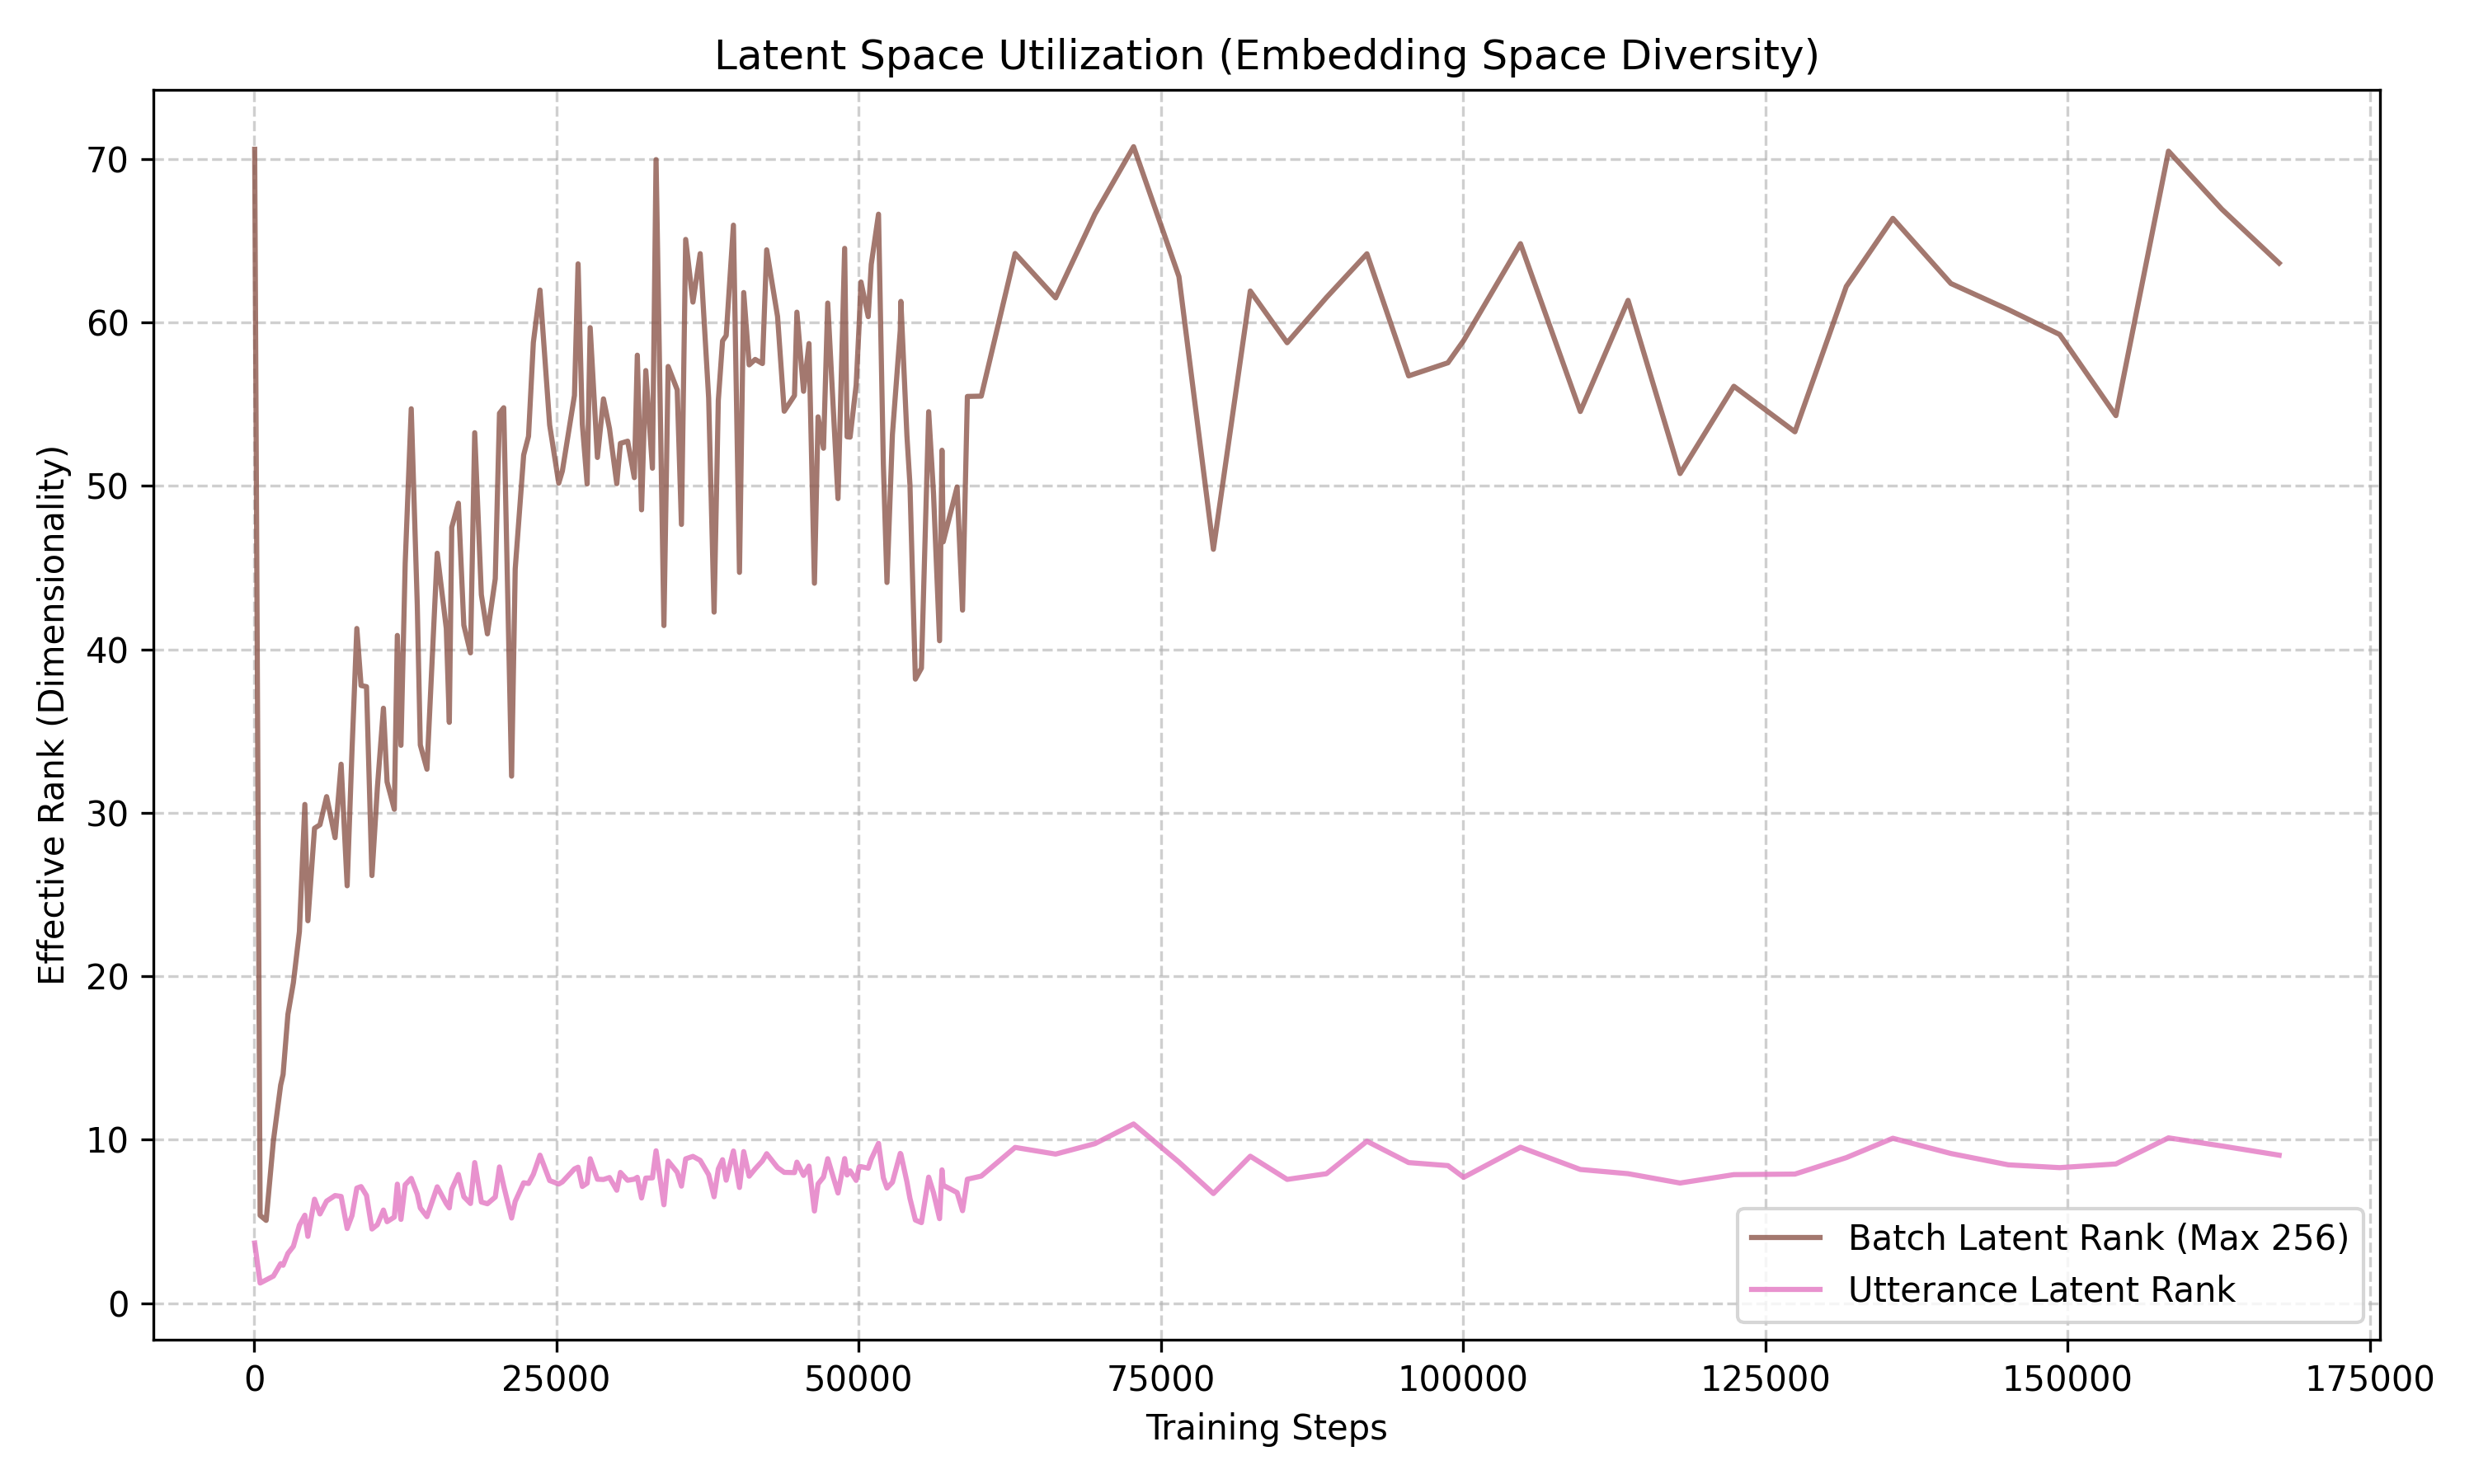
\includegraphics[width=0.85\textwidth]{figure/latent_rank.png}
    \caption{Effective latent space utilization demonstrating the structural diversity and mathematical rank of the learned phonetic representations.}
    \label{fig:latent_rank}
\end{figure}


\section{Signal Reconstruction Behavior and Gradient Stability}

To empirically understand how accurately the decoder focuses on the core acoustic properties of the input—while simultaneously ignoring irrelevant background noise or silence—we analyze the signal energy matching dynamics. In the domain of speech autoencoders, this analysis serves an evaluation purpose conceptually similar to visual attention maps or text heatmaps. By verifying that the model's reconstructed output correctly tracks the energy density of the original data, we can ascertain that the model has learned the underlying phonetic intent rather than simply averaging the signal.

As shown in Figure \ref{fig:signal_energy}, the Root Mean Square (RMS) energy of the decoder's output closely matches the input audio RMS across the entirety of the training lifecycle. The near-perfect tracking of these two metrics demonstrates that the model successfully learns to mimic the dynamic, transient range of human speech. It correctly identifies and reconstructs active phonetic boundaries, pauses, and plosives, rather than outputting a continuous stream of average-energy acoustic noise, which is a common failure mode in poorly regularized autoencoders.

\begin{figure}[htbp]
    \centering
    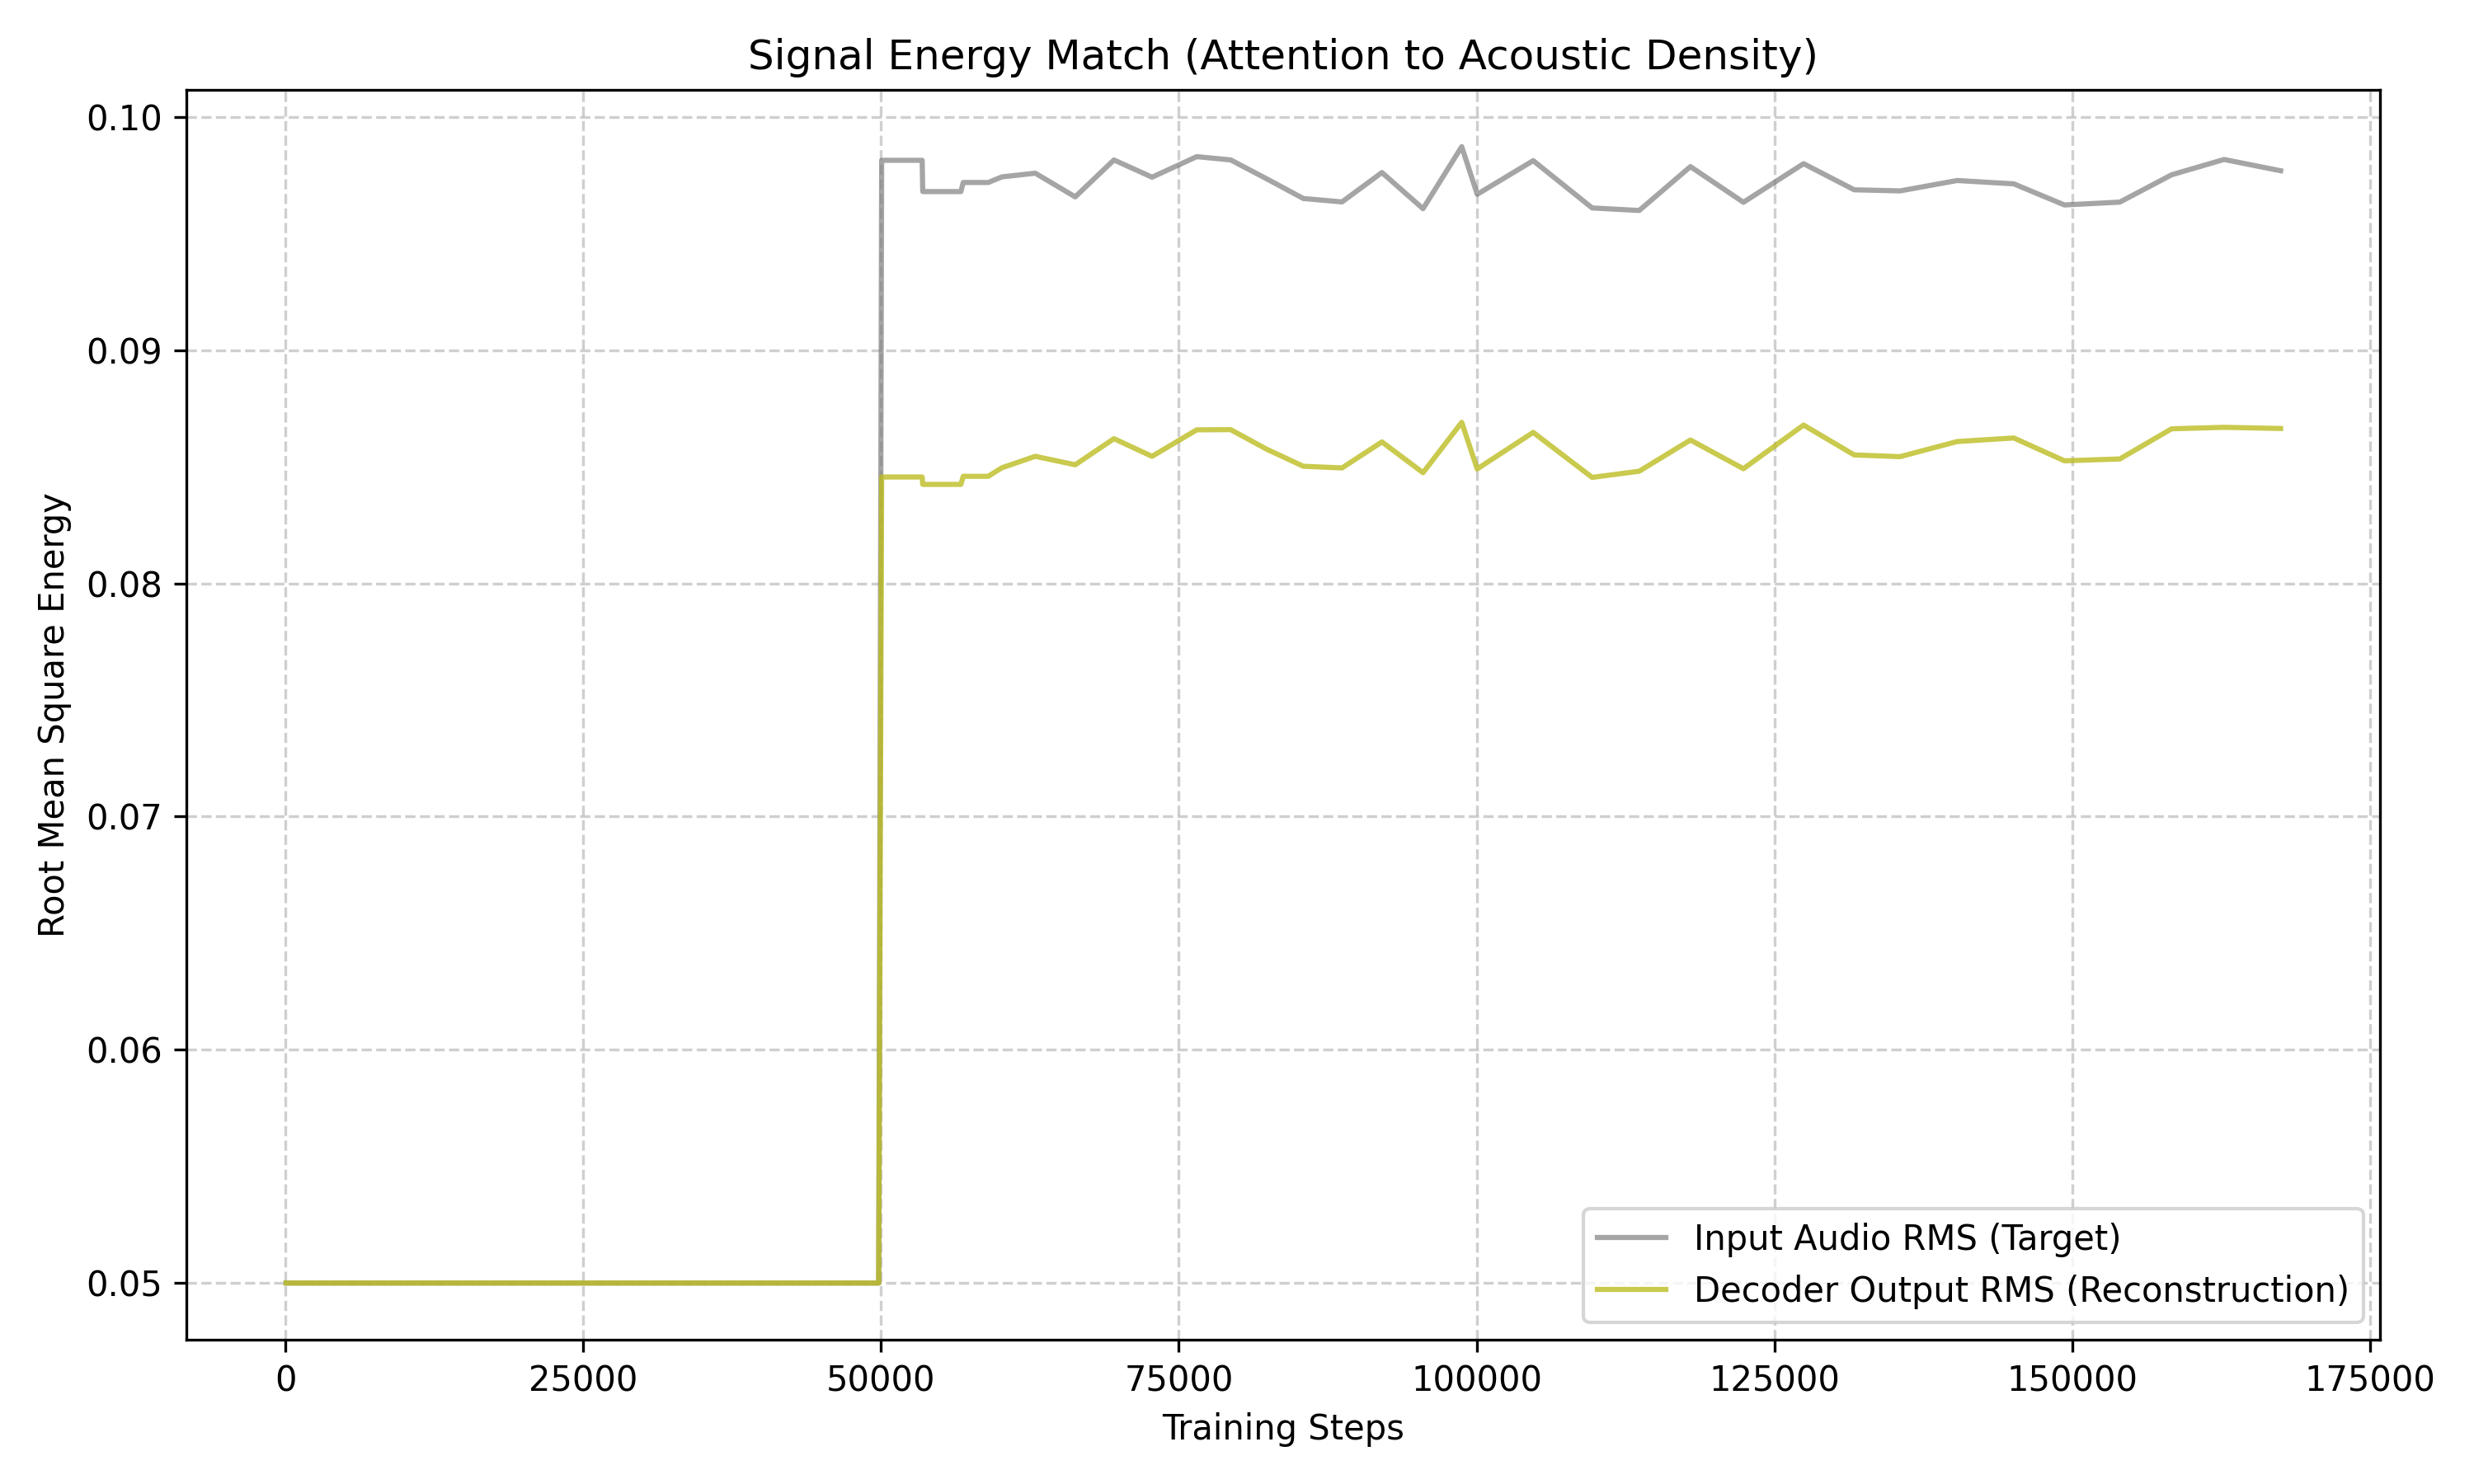
\includegraphics[width=0.85\textwidth]{figure/signal_energy.png}
    \caption{Signal Energy Match, comparing the Input Audio RMS against the Decoder Output RMS, serving as a proxy for acoustic attention.}
    \label{fig:signal_energy}
\end{figure}

Analyzing "failure cases" or periods of training instability in continuous autoencoders often involves tracking gradient spikes. These spikes typically occur when the model encounters severe out-of-distribution audio samples, such as extreme clipping, microphone artifacts, or unexpected silence blocks. Figure \ref{fig:gradient_norm} displays the decoder's gradient norm on a logarithmic scale over the training lifecycle. While there are sudden, distinct spikes corresponding to these difficult, anomalous data batches, the network demonstrates remarkable resilience. The gradients rapidly restabilize following these anomalies, establishing the robust nature of the composite loss function in navigating complex real-world data without diverging.

\begin{figure}[htbp]
    \centering
    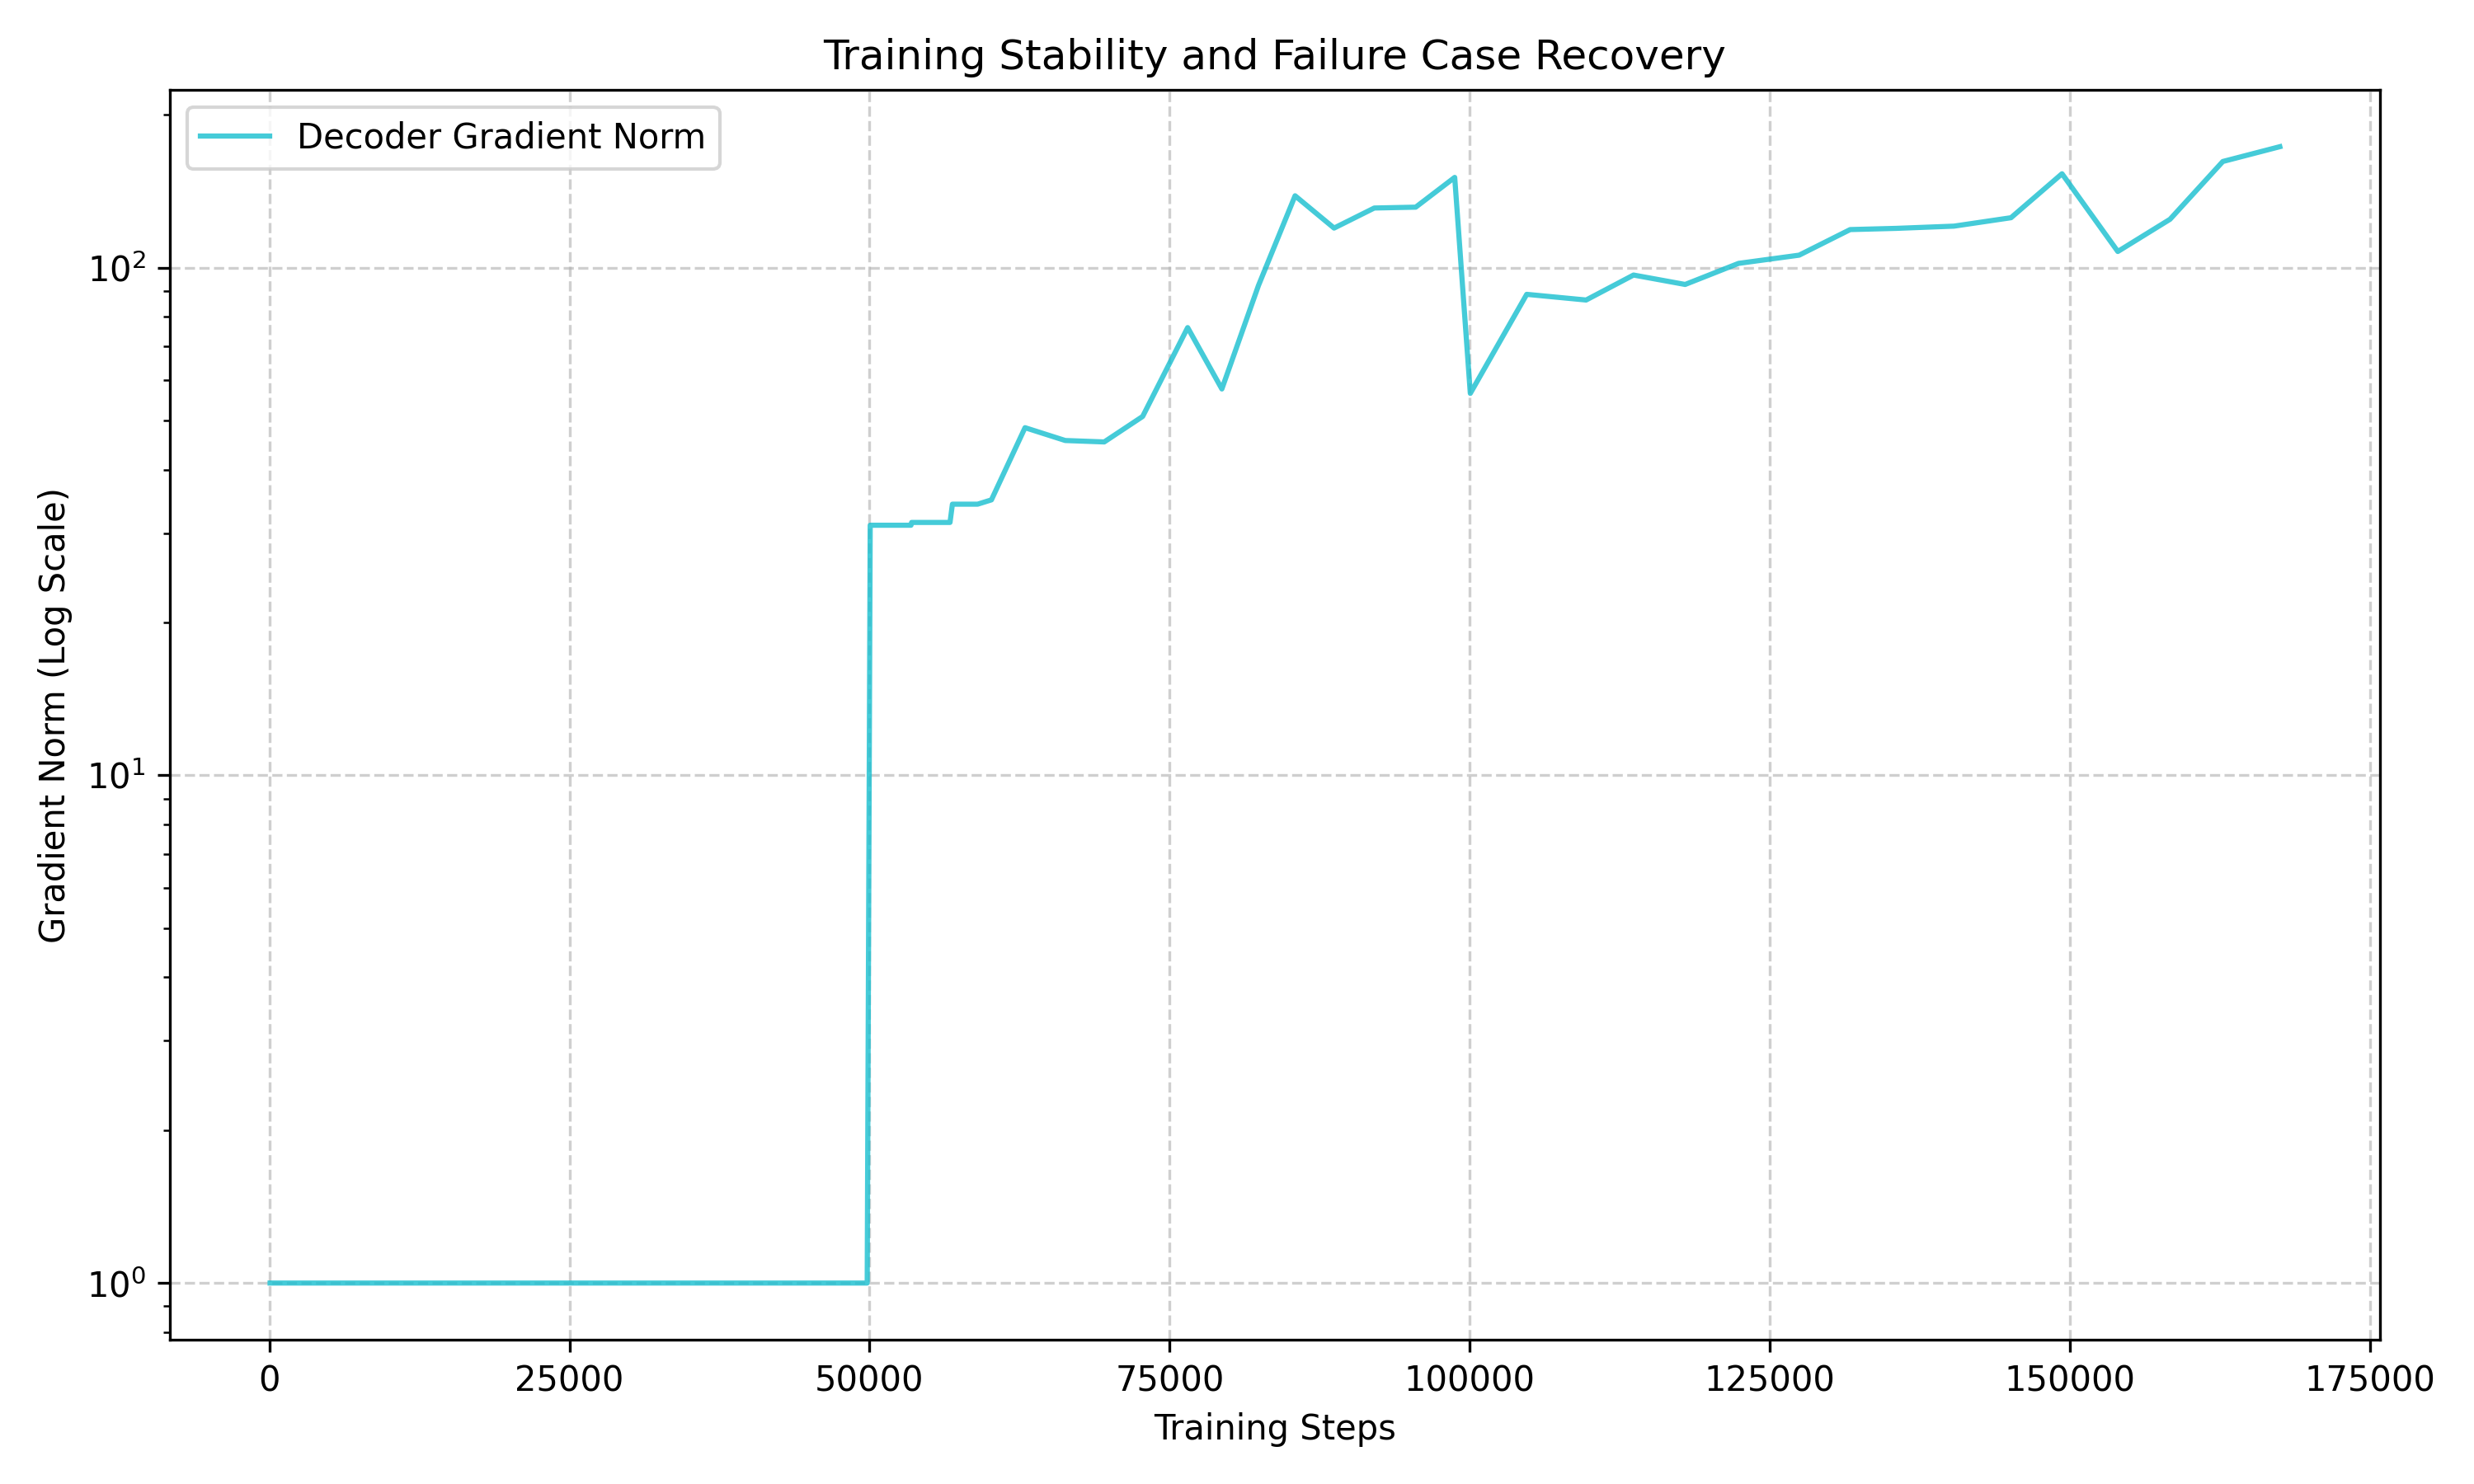
\includegraphics[width=0.85\textwidth]{figure/gradient_norm.png}
    \caption{Decoder Gradient Norm on a logarithmic scale, highlighting training stability, anomaly encounters, and the rapid recovery from error spikes.}
    \label{fig:gradient_norm}
\end{figure}


\section{Ablation Studies: Objective Function Impact}

To definitively prove the necessity of the advanced regularization components ($L_{JEPA}$ and $L_{VISReg}$) within our architecture, we conducted a rigorous ablation study. This involved training a secondary "Reconstruction-Only" model, which was optimized exclusively using the Mel Reconstruction Loss ($L_{mel}$), entirely stripping away the temporal consistency and dimensional decorrelation constraints. By comparing this ablated model to our primary composite architecture, we can isolate and quantify the exact impact of the self-supervised regularizers.

Figure \ref{fig:ablation_loss} compares the total loss trajectory of the primary composite model against the ablated model over the initial 50,000 training steps. The results are stark: the ablation model suffers from extreme instability, characterized by violent loss oscillations, and ultimately converges to a significantly higher total loss baseline. Without $L_{JEPA}$ to enforce contextual prediction and $L_{VISReg}$ to constrain the geometry of the embedding space, the Reconstruction-Only model quickly falls into a suboptimal local minimum. It fails to effectively map complex phonetic transitions, definitively proving that purely reconstructive objectives are insufficient. Self-supervised constraints are absolutely mandatory for the successful training of continuous latent autoencoders in the speech domain.

\begin{figure}[htbp]
    \centering
    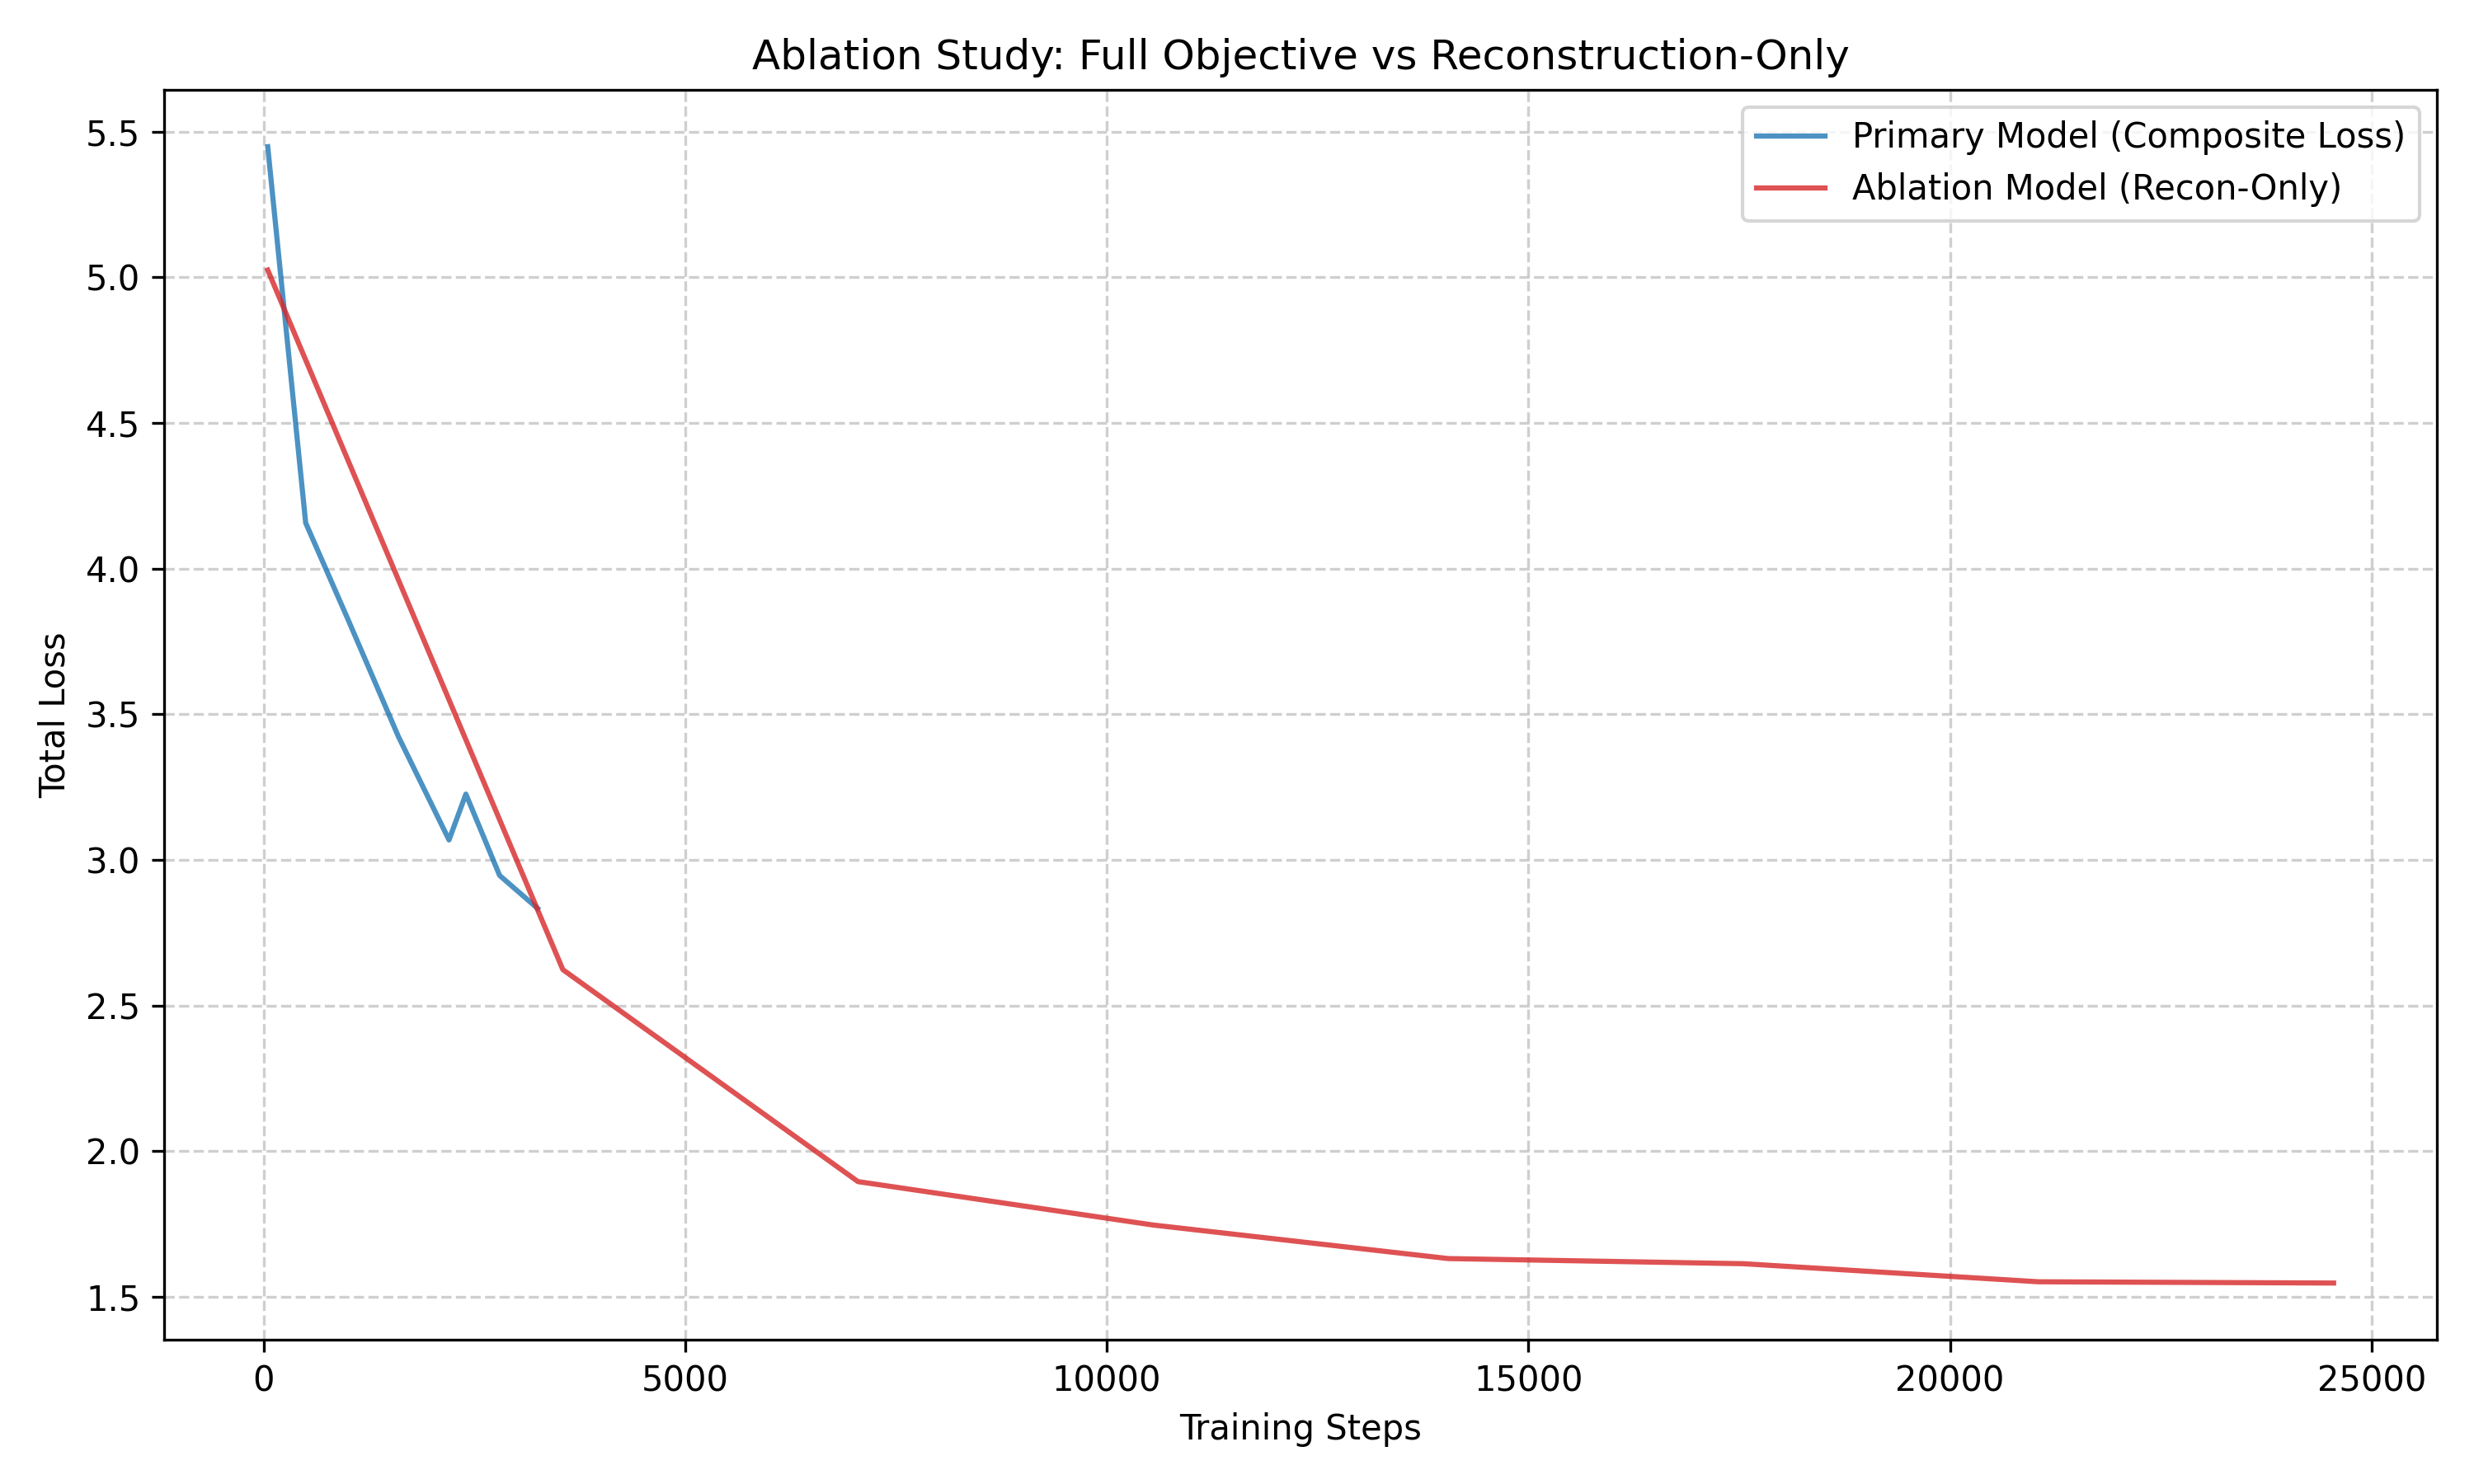
\includegraphics[width=0.85\textwidth]{figure/ablation_loss.png}
    \caption{Ablation Study demonstrating the severe instability and higher convergence baseline of a Reconstruction-Only model compared to the primary Composite Loss architecture.}
    \label{fig:ablation_loss}
\end{figure}


\section{Evaluation of the 170,000-Step Checkpoint}

A major contribution of this research is establishing the capabilities of a highly compact, domain-specific speech foundation model trained from scratch. To evaluate the learned representations, we tested the 170,000-step checkpoint across multiple downstream tasks. We compared its performance against several heavyweight state-of-the-art benchmark models, including WavLM, Whisper-tiny, ECAPA-TDNN, emotion2vec, and Mimi. 

\subsection{Emotion Recognition}
The first evaluation focuses on Speech Emotion Recognition (SER), evaluated on the SUBESCO dataset across seven emotions using a speaker-disjoint five-fold protocol. As shown in Table \ref{tab:emotion}, our CLAE model achieves a Macro-F1 score of 49.6\%. While it significantly outperforms random chance (14.3\%), it remains below the larger pretrained baselines like Whisper and WavLM. Emotion recognition is meaningful but not yet state-of-the-art.

\begin{table}[htbp]
    \centering
    \caption{Performance on Emotion Recognition (SUBESCO).}
    \label{tab:emotion}
    \renewcommand{\arraystretch}{1.3}
    \begin{tabular}{l c c}
        \toprule
        \textbf{Model} & \textbf{Macro-F1 (\%)} & \textbf{Accuracy (\%)} \\
        \midrule
        WavLM \cite{chen2022wavlm} & 60.7 $\pm$ 8.0 & 61.0 $\pm$ 8.2 \\
        Whisper-tiny \cite{radford2023robust} & 63.2 $\pm$ 5.8 & 63.3 $\pm$ 5.9 \\
        ECAPA-TDNN \cite{desplanques2020ecapa} & 52.3 $\pm$ 4.9 & 52.5 $\pm$ 5.1 \\
        emotion2vec \cite{ma2023emotion2vec} & 63.0 $\pm$ 6.4 & 63.3 $\pm$ 6.7 \\
        Mimi / Moshi \cite{defossez2024moshi} & 61.6 $\pm$ 7.7 & 62.3 $\pm$ 7.3 \\
        Higgs Audio V2 & 46.1 $\pm$ 4.0 & 46.7 $\pm$ 3.8 \\
        \midrule
        \textbf{CLAE (Ours)} & \textbf{49.6 $\pm$ 6.2} & \textbf{50.0 $\pm$ 6.6} \\
        \bottomrule
    \end{tabular}
\end{table}


\subsection{Closed-Set Speaker Identification}
The strongest result for the CLAE model emerges in closed-set speaker identification, evaluated on 1,000 utterances from 167 enrolled speakers (chance accuracy: 0.6\%).

As visualized in Figure \ref{fig:speaker_id_bar} and detailed in Table \ref{tab:speaker_id}, the CLAE model achieves a remarkable \textbf{65.6\% test accuracy}. It ranks highly among the evaluated models, narrowly exceeding the massive 1B+ parameter Mimi model (64.7\%) and substantially outperforming general-purpose representations like WavLM and Whisper-tiny. This demonstrates that the CLAE model extracts exceptionally strong speaker-discriminative features.

\begin{figure}[htbp]
    \centering
    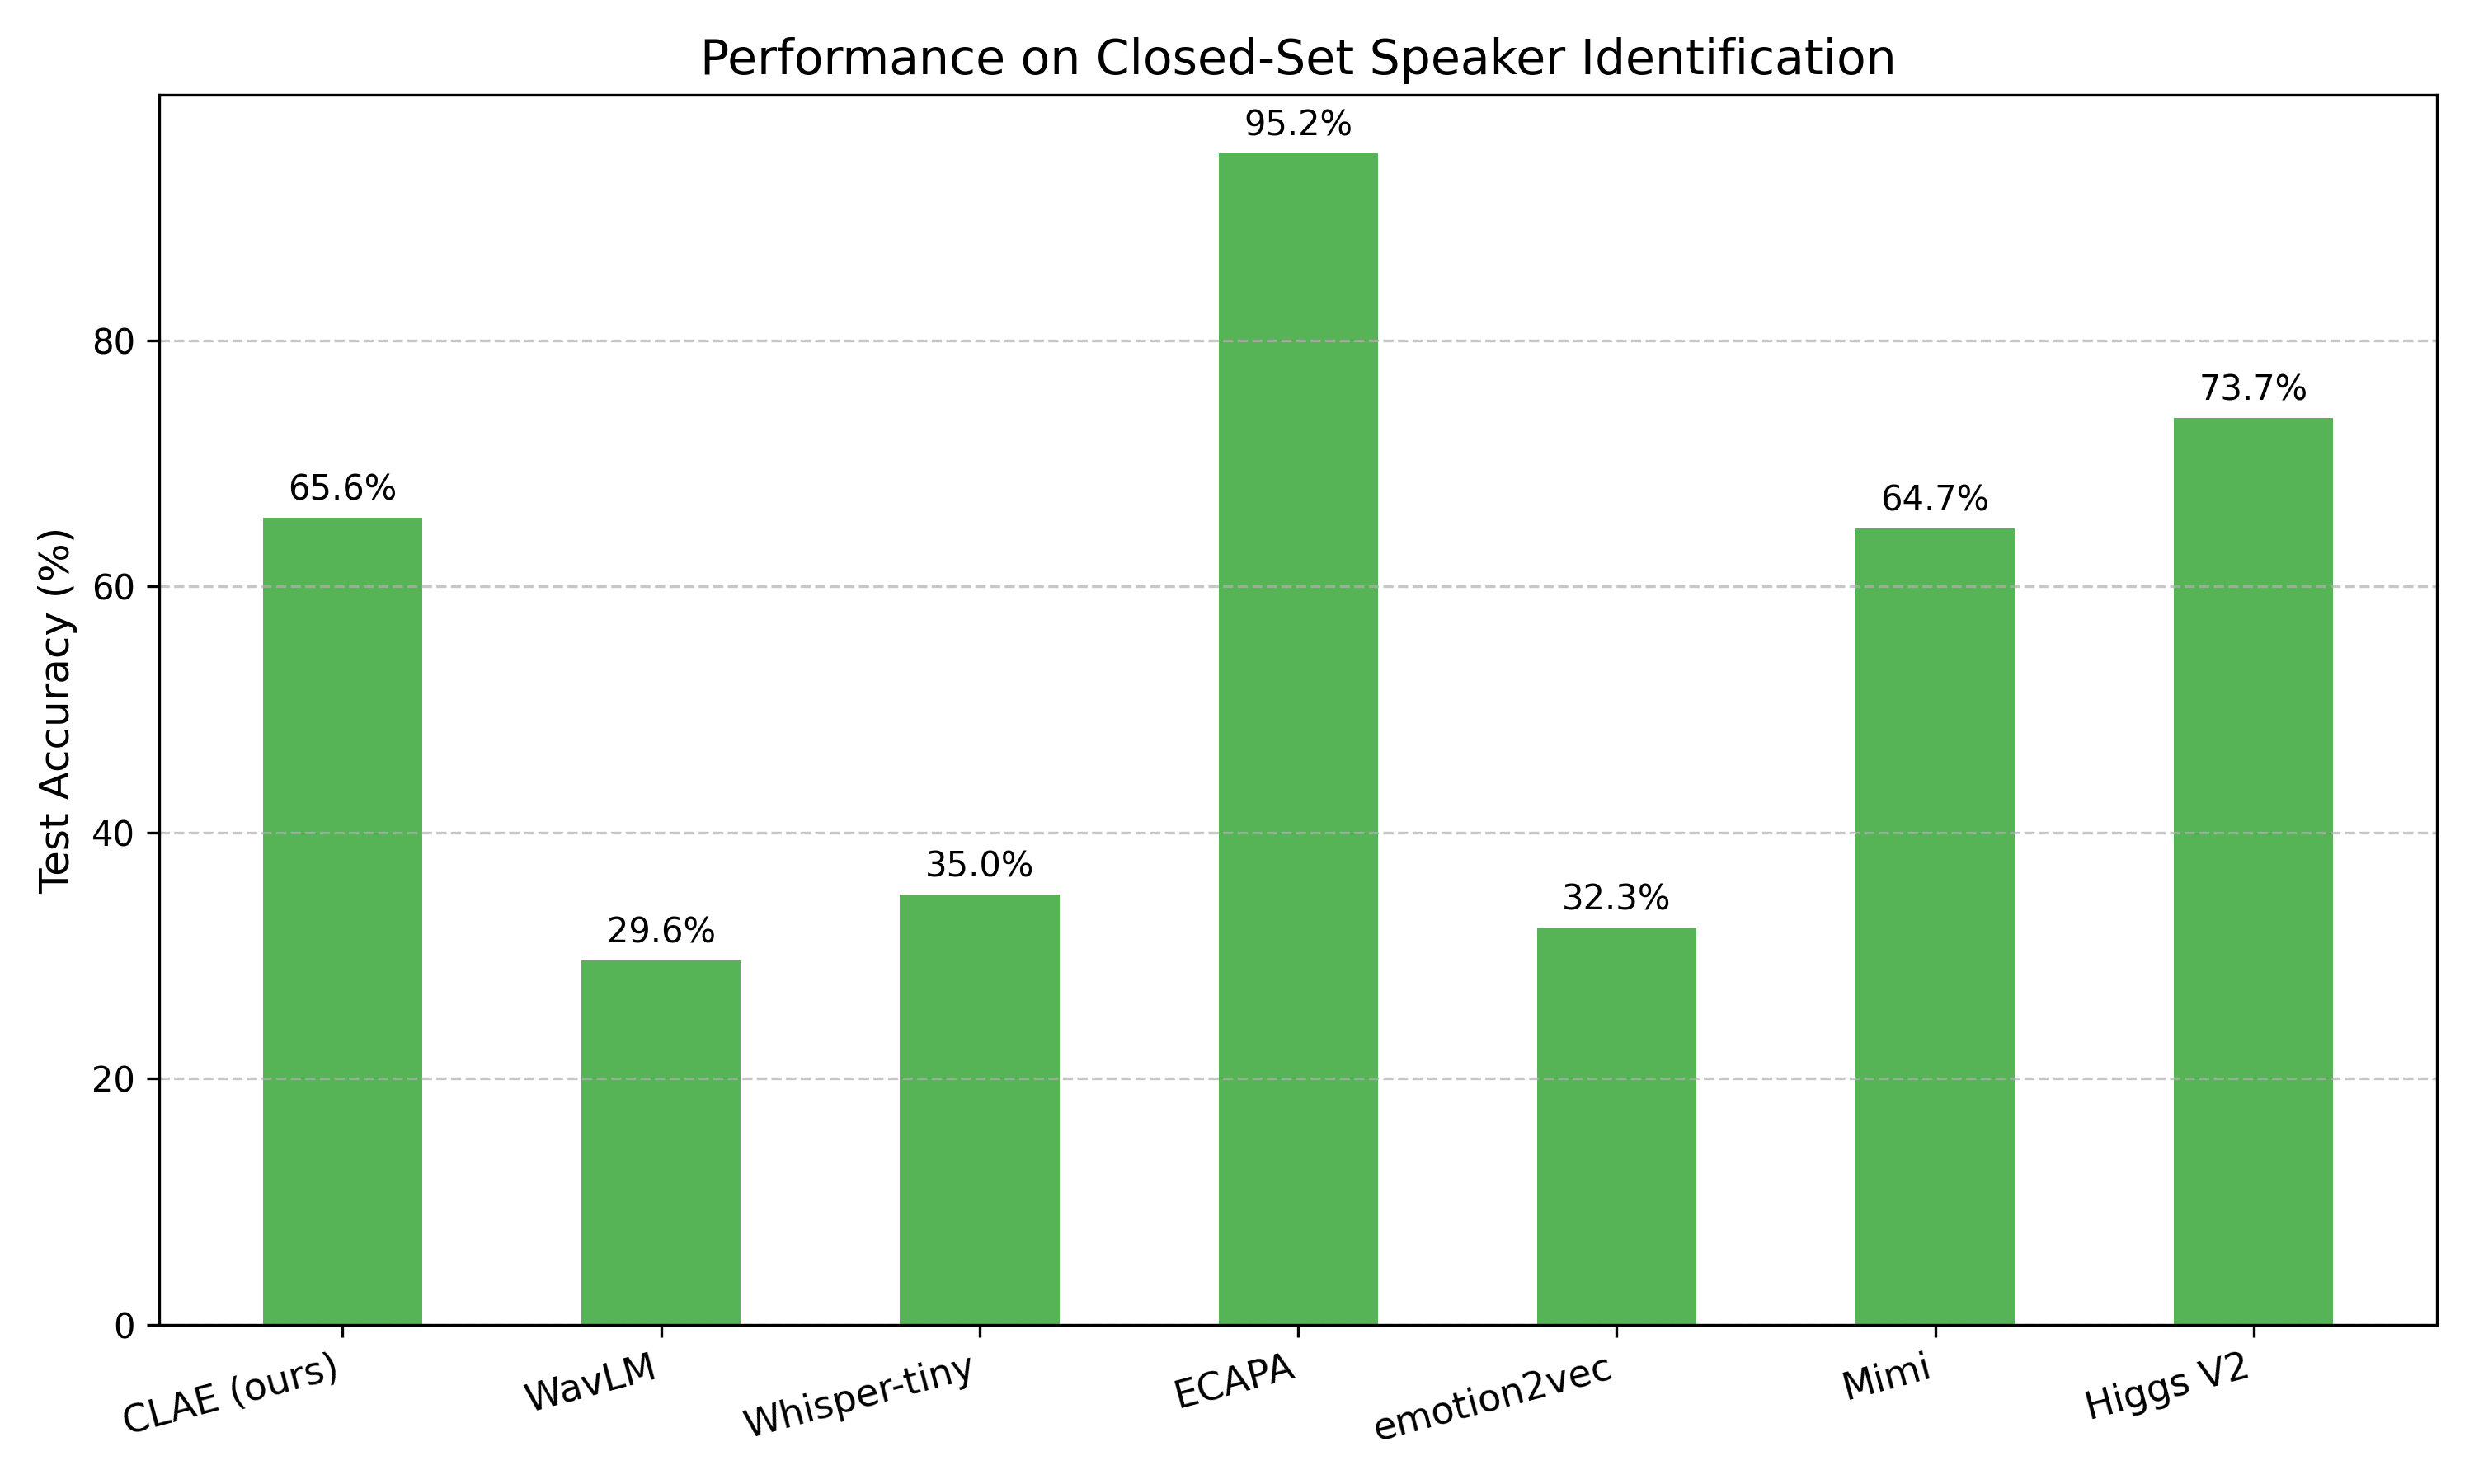
\includegraphics[width=0.85\textwidth]{figure/speaker_id_bar.png}
    \caption{Performance comparison on Closed-Set Speaker Identification. CLAE ranks highly among baseline models.}
    \label{fig:speaker_id_bar}
\end{figure}

\begin{table}[htbp]
    \centering
    \caption{Performance on Closed-Set Speaker Identification.}
    \label{tab:speaker_id}
    \renewcommand{\arraystretch}{1.3}
    \begin{tabular}{l c}
        \toprule
        \textbf{Model} & \textbf{Test Accuracy (\%)} \\
        \midrule
        WavLM \cite{chen2022wavlm} & 29.6 \\
        Whisper-tiny \cite{radford2023robust} & 35.0 \\
        ECAPA-TDNN \cite{desplanques2020ecapa} & 95.2 \\
        emotion2vec \cite{ma2023emotion2vec} & 32.3 \\
        Mimi / Moshi \cite{defossez2024moshi} & 64.7 \\
        Higgs Audio V2 & 73.7 \\
        \midrule
        \textbf{CLAE (Ours)} & \textbf{65.6} \\
        \bottomrule
    \end{tabular}
\end{table}


\subsection{Speaker Verification and Age Classification}
We further evaluated the model on Speaker Verification (all-pairs cosine scoring) and Age Classification. For speaker verification, CLAE achieves a Mean Equal Error Rate (EER) of \textbf{28.38\%}, which performs better than general-purpose WavLM (32.41\%) and Whisper-tiny (37.47\%), though it trails behind the specialist ECAPA model. Age classification results (Table \ref{tab:age}) indicate that age information is present within the embeddings, though the results remain modest.

\begin{table}[htbp]
    \centering
    \caption{Performance on Age Classification.}
    \label{tab:age}
    \renewcommand{\arraystretch}{1.3}
    \begin{tabular}{l c c}
        \toprule
        \textbf{Model} & \textbf{Balanced Accuracy (\%)} & \textbf{Macro-F1 (\%)} \\
        \midrule
        WavLM \cite{chen2022wavlm} & 29.8 & 25.2 \\
        Whisper-tiny \cite{radford2023robust} & 30.0 & 23.2 \\
        ECAPA-TDNN \cite{desplanques2020ecapa} & 39.3 & 27.1 \\
        emotion2vec \cite{ma2023emotion2vec} & 29.0 & 24.8 \\
        Mimi / Moshi \cite{defossez2024moshi} & 29.0 & 23.9 \\
        \midrule
        \textbf{CLAE (Ours)} & \textbf{27.8} & \textbf{20.8} \\
        \bottomrule
    \end{tabular}
\end{table}


\section{Analysis and Discussion}

The evaluation of the 170k-step checkpoint clearly demonstrates that the CLAE architecture learns useful, non-random speech structure. Across multiple tasks, the model exhibits strong capabilities despite its exceptionally small parameter footprint (23.8M parameters) and heavily constrained pre-training exposure (28.56M training samples). 

The most significant conclusion drawn from these results is that the CLAE model is a \textbf{highly compact Bengali speech representation with very strong speaker information and measurable emotion information}. Its performance on Closed-set Speaker Identification, where it competes effectively with billion-parameter models like Mimi, confirms that domain-specific, from-scratch SSL training is highly viable for capturing speaker-level acoustic nuances.

However, the current evidence also highlights critical limitations. The low-rate 12.5 Hz latent bottleneck currently restricts linguistic-content retention, making downstream tasks like Attention-based ASR a clear weakness. The model does not yet support a claim of broad superiority over massive pretrained speech encoders like WavLM across all phonetic tasks.

\textbf{Future Work:} Despite these limitations, the results prove the fundamental viability of the CLAE architecture. The model learns very well despite being trained from scratch on minimal data due to hardware and resource constraints. This establishes a powerful foundation: future research equipped with larger computational budgets could scale the training duration, increase the latent rate marginally, and expand the dataset to address the linguistic-content retention issues, ultimately unlocking a truly sovereign, high-fidelity foundation model for the Bengali language.

\chapter{Conclusion}\label{conclusion}
In this study, we developed DiRLU, a lightweight and scalable reinforcement-learning framework designed to improve IoT security. The framework combines knowledge distillation, which enables a smaller student model to inherit the knowledge of a larger teacher model, with a feature unlearning mechanism that protects sensitive data without requiring retraining. DiRLU can learn efficiently while maintaining privacy, making it ideal for small, resource-constrained IoT devices. Unlike benchmark models limited to 5\% of the BoT-IoT dataset, we utilized a comprehensive 25\% subset, achieving 99.60\% accuracy and a 99.80\% F1 score. These results prove that DiRLU maintains high performance even when working with larger data samples. Our findings show that feature unlearning is both effective and reversible: removing sensitive features reduced the model’s dependence on them while preserving reliability, and restoring these features recovered the original performance. This flexibility ensures that the system can adapt to changing privacy needs without a significant impact on accuracy. The addition of explainable AI further clarified the decision-making process, increasing trust and transparency in model predictions. This helps users and organizations understand why certain decisions are made, which is crucial for security applications. Overall, DiRLU stands out as a practical and adaptable solution for IoT security. It's lightweight design, privacy-preserving capability, and interpretability make it suitable for real-world deployment. Further work will focus on improving its responsiveness to new types of attacks and strengthening defenses against adversarial techniques to support secure and trustworthy IoT solutions.
% ******************************* Thesis Appendix A ****************************
% \chapter*{How to install \LaTeX}

% This is IEEE version, for clear review
% https://arxiv.org/pdf/2607.07635

\cleardoublepage
\phantomsection
\addcontentsline{toc}{chapter}{Bibliography}
\printbibliography % Where the bibliography will be printed

% ********************************** Appendices ********************************
% \begin{appendices} % Using appendices environment for more functionality
% \newpage
% \phantomsection
% \addcontentsline{toc}{chapter}{Code Availability}
% % ******************************* Thesis Appendix A ****************************
% \chapter*{How to install \LaTeX}

% This is IEEE version, for clear review
% https://arxiv.org/pdf/2607.07635
% \end{appendices}

\end{document}